% Generated by Sphinx.
\def\sphinxdocclass{report}
\documentclass[letterpaper,10pt,english]{sphinxmanual}
\usepackage[utf8]{inputenc}
\DeclareUnicodeCharacter{00A0}{\nobreakspace}
\usepackage[T1]{fontenc}
\usepackage{babel}
\usepackage{times}
\usepackage[Sonny]{fncychap}
\usepackage{longtable}
\usepackage{sphinx}
\usepackage{multirow}


\title{Zephir Documentation}
\date{September 03, 2013}
\release{0.2.0a}
\author{Zephir Team}
\newcommand{\sphinxlogo}{}
\renewcommand{\releasename}{Release}
\makeindex

\makeatletter
\def\PYG@reset{\let\PYG@it=\relax \let\PYG@bf=\relax%
    \let\PYG@ul=\relax \let\PYG@tc=\relax%
    \let\PYG@bc=\relax \let\PYG@ff=\relax}
\def\PYG@tok#1{\csname PYG@tok@#1\endcsname}
\def\PYG@toks#1+{\ifx\relax#1\empty\else%
    \PYG@tok{#1}\expandafter\PYG@toks\fi}
\def\PYG@do#1{\PYG@bc{\PYG@tc{\PYG@ul{%
    \PYG@it{\PYG@bf{\PYG@ff{#1}}}}}}}
\def\PYG#1#2{\PYG@reset\PYG@toks#1+\relax+\PYG@do{#2}}

\def\PYG@tok@gd{\def\PYG@tc##1{\textcolor[rgb]{0.63,0.00,0.00}{##1}}}
\def\PYG@tok@gu{\let\PYG@bf=\textbf\def\PYG@tc##1{\textcolor[rgb]{0.50,0.00,0.50}{##1}}}
\def\PYG@tok@gt{\def\PYG@tc##1{\textcolor[rgb]{0.00,0.25,0.82}{##1}}}
\def\PYG@tok@gs{\let\PYG@bf=\textbf}
\def\PYG@tok@gr{\def\PYG@tc##1{\textcolor[rgb]{1.00,0.00,0.00}{##1}}}
\def\PYG@tok@cm{\let\PYG@it=\textit\def\PYG@tc##1{\textcolor[rgb]{0.25,0.50,0.56}{##1}}}
\def\PYG@tok@vg{\def\PYG@tc##1{\textcolor[rgb]{0.73,0.38,0.84}{##1}}}
\def\PYG@tok@m{\def\PYG@tc##1{\textcolor[rgb]{0.13,0.50,0.31}{##1}}}
\def\PYG@tok@mh{\def\PYG@tc##1{\textcolor[rgb]{0.13,0.50,0.31}{##1}}}
\def\PYG@tok@cs{\def\PYG@tc##1{\textcolor[rgb]{0.25,0.50,0.56}{##1}}\def\PYG@bc##1{\colorbox[rgb]{1.00,0.94,0.94}{##1}}}
\def\PYG@tok@ge{\let\PYG@it=\textit}
\def\PYG@tok@vc{\def\PYG@tc##1{\textcolor[rgb]{0.73,0.38,0.84}{##1}}}
\def\PYG@tok@il{\def\PYG@tc##1{\textcolor[rgb]{0.13,0.50,0.31}{##1}}}
\def\PYG@tok@go{\def\PYG@tc##1{\textcolor[rgb]{0.19,0.19,0.19}{##1}}}
\def\PYG@tok@cp{\def\PYG@tc##1{\textcolor[rgb]{0.00,0.44,0.13}{##1}}}
\def\PYG@tok@gi{\def\PYG@tc##1{\textcolor[rgb]{0.00,0.63,0.00}{##1}}}
\def\PYG@tok@gh{\let\PYG@bf=\textbf\def\PYG@tc##1{\textcolor[rgb]{0.00,0.00,0.50}{##1}}}
\def\PYG@tok@ni{\let\PYG@bf=\textbf\def\PYG@tc##1{\textcolor[rgb]{0.84,0.33,0.22}{##1}}}
\def\PYG@tok@nl{\let\PYG@bf=\textbf\def\PYG@tc##1{\textcolor[rgb]{0.00,0.13,0.44}{##1}}}
\def\PYG@tok@nn{\let\PYG@bf=\textbf\def\PYG@tc##1{\textcolor[rgb]{0.05,0.52,0.71}{##1}}}
\def\PYG@tok@no{\def\PYG@tc##1{\textcolor[rgb]{0.38,0.68,0.84}{##1}}}
\def\PYG@tok@na{\def\PYG@tc##1{\textcolor[rgb]{0.25,0.44,0.63}{##1}}}
\def\PYG@tok@nb{\def\PYG@tc##1{\textcolor[rgb]{0.00,0.44,0.13}{##1}}}
\def\PYG@tok@nc{\let\PYG@bf=\textbf\def\PYG@tc##1{\textcolor[rgb]{0.05,0.52,0.71}{##1}}}
\def\PYG@tok@nd{\let\PYG@bf=\textbf\def\PYG@tc##1{\textcolor[rgb]{0.33,0.33,0.33}{##1}}}
\def\PYG@tok@ne{\def\PYG@tc##1{\textcolor[rgb]{0.00,0.44,0.13}{##1}}}
\def\PYG@tok@nf{\def\PYG@tc##1{\textcolor[rgb]{0.02,0.16,0.49}{##1}}}
\def\PYG@tok@si{\let\PYG@it=\textit\def\PYG@tc##1{\textcolor[rgb]{0.44,0.63,0.82}{##1}}}
\def\PYG@tok@s2{\def\PYG@tc##1{\textcolor[rgb]{0.25,0.44,0.63}{##1}}}
\def\PYG@tok@vi{\def\PYG@tc##1{\textcolor[rgb]{0.73,0.38,0.84}{##1}}}
\def\PYG@tok@nt{\let\PYG@bf=\textbf\def\PYG@tc##1{\textcolor[rgb]{0.02,0.16,0.45}{##1}}}
\def\PYG@tok@nv{\def\PYG@tc##1{\textcolor[rgb]{0.73,0.38,0.84}{##1}}}
\def\PYG@tok@s1{\def\PYG@tc##1{\textcolor[rgb]{0.25,0.44,0.63}{##1}}}
\def\PYG@tok@gp{\let\PYG@bf=\textbf\def\PYG@tc##1{\textcolor[rgb]{0.78,0.36,0.04}{##1}}}
\def\PYG@tok@sh{\def\PYG@tc##1{\textcolor[rgb]{0.25,0.44,0.63}{##1}}}
\def\PYG@tok@ow{\let\PYG@bf=\textbf\def\PYG@tc##1{\textcolor[rgb]{0.00,0.44,0.13}{##1}}}
\def\PYG@tok@sx{\def\PYG@tc##1{\textcolor[rgb]{0.78,0.36,0.04}{##1}}}
\def\PYG@tok@bp{\def\PYG@tc##1{\textcolor[rgb]{0.00,0.44,0.13}{##1}}}
\def\PYG@tok@c1{\let\PYG@it=\textit\def\PYG@tc##1{\textcolor[rgb]{0.25,0.50,0.56}{##1}}}
\def\PYG@tok@kc{\let\PYG@bf=\textbf\def\PYG@tc##1{\textcolor[rgb]{0.00,0.44,0.13}{##1}}}
\def\PYG@tok@c{\let\PYG@it=\textit\def\PYG@tc##1{\textcolor[rgb]{0.25,0.50,0.56}{##1}}}
\def\PYG@tok@mf{\def\PYG@tc##1{\textcolor[rgb]{0.13,0.50,0.31}{##1}}}
\def\PYG@tok@err{\def\PYG@bc##1{\fcolorbox[rgb]{1.00,0.00,0.00}{1,1,1}{##1}}}
\def\PYG@tok@kd{\let\PYG@bf=\textbf\def\PYG@tc##1{\textcolor[rgb]{0.00,0.44,0.13}{##1}}}
\def\PYG@tok@ss{\def\PYG@tc##1{\textcolor[rgb]{0.32,0.47,0.09}{##1}}}
\def\PYG@tok@sr{\def\PYG@tc##1{\textcolor[rgb]{0.14,0.33,0.53}{##1}}}
\def\PYG@tok@mo{\def\PYG@tc##1{\textcolor[rgb]{0.13,0.50,0.31}{##1}}}
\def\PYG@tok@mi{\def\PYG@tc##1{\textcolor[rgb]{0.13,0.50,0.31}{##1}}}
\def\PYG@tok@kn{\let\PYG@bf=\textbf\def\PYG@tc##1{\textcolor[rgb]{0.00,0.44,0.13}{##1}}}
\def\PYG@tok@o{\def\PYG@tc##1{\textcolor[rgb]{0.40,0.40,0.40}{##1}}}
\def\PYG@tok@kr{\let\PYG@bf=\textbf\def\PYG@tc##1{\textcolor[rgb]{0.00,0.44,0.13}{##1}}}
\def\PYG@tok@s{\def\PYG@tc##1{\textcolor[rgb]{0.25,0.44,0.63}{##1}}}
\def\PYG@tok@kp{\def\PYG@tc##1{\textcolor[rgb]{0.00,0.44,0.13}{##1}}}
\def\PYG@tok@w{\def\PYG@tc##1{\textcolor[rgb]{0.73,0.73,0.73}{##1}}}
\def\PYG@tok@kt{\def\PYG@tc##1{\textcolor[rgb]{0.56,0.13,0.00}{##1}}}
\def\PYG@tok@sc{\def\PYG@tc##1{\textcolor[rgb]{0.25,0.44,0.63}{##1}}}
\def\PYG@tok@sb{\def\PYG@tc##1{\textcolor[rgb]{0.25,0.44,0.63}{##1}}}
\def\PYG@tok@k{\let\PYG@bf=\textbf\def\PYG@tc##1{\textcolor[rgb]{0.00,0.44,0.13}{##1}}}
\def\PYG@tok@se{\let\PYG@bf=\textbf\def\PYG@tc##1{\textcolor[rgb]{0.25,0.44,0.63}{##1}}}
\def\PYG@tok@sd{\let\PYG@it=\textit\def\PYG@tc##1{\textcolor[rgb]{0.25,0.44,0.63}{##1}}}

\def\PYGZbs{\char`\\}
\def\PYGZus{\char`\_}
\def\PYGZob{\char`\{}
\def\PYGZcb{\char`\}}
\def\PYGZca{\char`\^}
\def\PYGZsh{\char`\#}
\def\PYGZpc{\char`\%}
\def\PYGZdl{\char`\$}
\def\PYGZti{\char`\~}
% for compatibility with earlier versions
\def\PYGZat{@}
\def\PYGZlb{[}
\def\PYGZrb{]}
\makeatother

\begin{document}

\maketitle
\tableofcontents
\phantomsection\label{index::doc}



\chapter{Reference}
\label{index:zephir-language}\label{index:reference}

\section{Welcome!}
\label{welcome:welcome}\label{welcome::doc}
Welcome to Zephir, an open source, high level/domain specific language
designed to ease the creation and maintainability of extensions for PHP
with a focus on type and memory safety.


\subsection{Some features}
\label{welcome:some-features}
Zephir's main features are:

\begin{tabulary}{\linewidth}{|L|L|}
\hline

Type system
 & 
dynamic/static
\\\hline

Memory safety
 & 
pointers or direct memory management aren't allowed
\\\hline

Compilation model
 & 
ahead of time
\\\hline

Memory model
 & 
task-local garbage collection
\\\hline
\end{tabulary}



\subsection{A small taste}
\label{welcome:a-small-taste}
The following code registers a class with a method that filters variables returning its
alphabetic characters:

\begin{Verbatim}[commandchars=\\\{\}]
\PYG{n+nx}{namespace} \PYG{n+nx}{MyLibrary}\PYG{p}{;}

\PYG{c+cm}{/**}
\PYG{c+cm}{ * Filter}
\PYG{c+cm}{ */}
\PYG{k+kr}{class} \PYG{n+nx}{Filter}
\PYG{p}{\PYGZob{}}
    \PYG{c+cm}{/**}
\PYG{c+cm}{     * Filters a string returning its alpha characters}
\PYG{c+cm}{     *}
\PYG{c+cm}{     * @param string str}
\PYG{c+cm}{     */}
    \PYG{k+kr}{public} \PYG{k+kd}{function} \PYG{n+nx}{alpha}\PYG{p}{(}\PYG{n+nx}{string} \PYG{n+nx}{str}\PYG{p}{)}
    \PYG{p}{\PYGZob{}}
        \PYG{k+kr}{char} \PYG{n+nx}{ch}\PYG{p}{;} \PYG{n+nx}{string} \PYG{n+nx}{filtered} \PYG{o}{=} \PYG{l+s+s2}{""}\PYG{p}{;}

        \PYG{k}{for} \PYG{n+nx}{ch} \PYG{k}{in} \PYG{n+nx}{str} \PYG{p}{\PYGZob{}}
           \PYG{k}{if} \PYG{p}{(}\PYG{n+nx}{ch} \PYG{o}{\textgreater{}=} \PYG{l+s+s1}{'a'} \PYG{o}{\&\&} \PYG{n+nx}{ch} \PYG{o}{\textless{}=} \PYG{l+s+s1}{'z'}\PYG{p}{)} \PYG{o}{\textbar{}\textbar{}} \PYG{p}{(}\PYG{n+nx}{ch} \PYG{o}{\textgreater{}=} \PYG{l+s+s1}{'A'} \PYG{o}{\&\&} \PYG{n+nx}{ch} \PYG{o}{\textless{}=} \PYG{l+s+s1}{'Z'}\PYG{p}{)} \PYG{p}{\PYGZob{}}
              \PYG{n+nx}{let} \PYG{n+nx}{filtered} \PYG{p}{.}\PYG{o}{=} \PYG{n+nx}{ch}\PYG{p}{;}
           \PYG{p}{\PYGZcb{}}
        \PYG{p}{\PYGZcb{}}

        \PYG{k}{return} \PYG{n+nx}{filtered}\PYG{p}{;}
    \PYG{p}{\PYGZcb{}}
\PYG{p}{\PYGZcb{}}
\end{Verbatim}

The class can be used from PHP as follows:

\begin{Verbatim}[commandchars=\\\{\}]
\PYG{c+cp}{\textless{}?php}

\PYG{n+nv}{\PYGZdl{}filter} \PYG{o}{=} \PYG{k}{new} \PYG{n+nx}{MyLibrary\PYGZbs{}Filter}\PYG{p}{();}
\PYG{k}{echo} \PYG{n+nv}{\PYGZdl{}filter}\PYG{o}{-\textgreater{}}\PYG{n+na}{alpha}\PYG{p}{(}\PYG{l+s+s2}{"}\PYG{l+s+s2}{01he}\PYG{l+s+si}{\PYGZdl{}l}\PYG{l+s+s2}{.lo?/1}\PYG{l+s+s2}{"}\PYG{p}{);} \PYG{c+c1}{// prints hello}
\end{Verbatim}


\section{Why Zephir?}
\label{motivation:why-zephir}\label{motivation::doc}
Today’s PHP applications must balance a number of concerns including stability, performance and functionality.
Every PHP application is based on a set of common components that are also base for most of the application.

These common components are libraries/frameworks or a combination of them. Once installed, frameworks rarely
change, being the foundation of the application they must be highly functional and also very fast.

Gettting fast and robust libraries can be complicated due to high levels of abstraction that are
typically implemented on them. Given the condition that base libraries or frameworks rarely change,
there is an opportunity to build extensions that provide this functionality taking advantage of the
compilation improving performance and resource consumption.

With Zephir you can implement object-oriented libraries/frameworks/applications that can be used from
PHP gaining important seconds that can make your application faster while improving the user experience.


\subsection{If You Are a PHP Programmer...}
\label{motivation:if-you-are-a-php-programmer}
PHP is one of the most popular languages in use for the development of web applications.
Dynamically typed and interpreted languages like PHP offer very high productivity due to their flexibility.

Since version 4 and then 5, PHP is based on the Zend Engine implementation. This is a virtual machine
that executes the PHP code from its bytecode representation. Zend Engine is almost present in every
PHP installation in the world. With Zephir you can create extensions for PHP running under the
Zend Engine.

PHP is hosting Zephir, so they obviously have a lot of similarities, however, they have
important differences that give Zephir its own personality. For example, Zephir is more strict
and it could be make you less productive compared to PHP due to the compilation step.


\subsection{If You Are a C Programmer...}
\label{motivation:if-you-are-a-c-programmer}
C is one of the most powerful and popular languages ever created. In fact, PHP is written in C,
which is one of the reasons why PHP extensions are available for it. C gives you the freedom to
manage memory, use low level types and even inline assembly routines.

However, developing big applications in C can take much longer than expected compared to PHP or Zephir
and some errors can be tricky to find if you aren't an experienced developer.

Zephir was designed to be safe, so it doesn't implement pointers or manual memory management, so
if you're a C programmer, you will feel Zephir less powerful but more friendly than C.


\subsection{Compilation vs Interpretation}
\label{motivation:compilation-vs-interpretation}
Compilation usually slows the development down, you will need a bit more of patience to make your
code compiled before see it running. Moreover, the interpretation tends to reduce the performance
in favor of productivity. In some cases there is no any noticeable difference between the speed of the
interpreted and compiled code.

Zephir requires compilation of your code, however the functionality is used from PHP that is interpreted.

Once the code is compiled is not necessary to do so, however, interpreted code is interpreted
each time it is run. A developer can decide which parts of your application should be in Zephir and which not.


\subsection{Statically Typed Versus Dynamically Typed Languages}
\label{motivation:statically-typed-versus-dynamically-typed-languages}
In general speaking, in a static typed language, a variable is bound to a particular type for its lifetime.
Its type can’t be changed and it can only reference type-compatible instances and operations.
Languages like C/C++ were implemented with the scheme:

\begin{Verbatim}[commandchars=\\\{\}]
\PYG{k+kt}{int} \PYG{n}{a} \PYG{o}{=} \PYG{l+m+mi}{0}\PYG{p}{;}
\PYG{n}{a} \PYG{o}{=} \PYG{l+s}{"}\PYG{l+s}{hello}\PYG{l+s}{"}\PYG{p}{;} \PYG{c+c1}{// not allowed}
\end{Verbatim}

In dynamic typing, the type is bound to the value, not the variable. So, a variable might refer
to a value of a type, then be reassigned later to a value of an unrelated type. Javascript/PHP are examples of
a dynamic typed language:

\begin{Verbatim}[commandchars=\\\{\}]
\PYG{k+kd}{var} \PYG{n+nx}{a} \PYG{o}{=} \PYG{l+m+mi}{0}\PYG{p}{;}
\PYG{n+nx}{a} \PYG{o}{=} \PYG{l+s+s2}{"hello"}\PYG{p}{;} \PYG{c+c1}{// allowed}
\end{Verbatim}

Despite their productivity advantages, dynamic languages may not be the best choices for all applications,
particularly for very large code bases and high-performance applications.

Optimizing the performance of a dynamic language like PHP is more challenging than for a static language like C.
In a static language, optimizers can exploit the type information to make decisions. In a dynamic language,
fewer such clues are available for the optimizer, making optimization choices harder.

While recent advancements in optimizations for dynamic languages are promising (like JIT compilation),
they lag behind the state of the art for static languages. So, if you require very high performance,
static languages are probably a safer choice.

Another small benefit of static languages is the extra checking the compiler performs.
A compiler can’t find logic errors, which are far more significant,
but a compiler can find errors in advance that in a dynamic language only can be
found in runtime.

Zephir is both statically and dynamically typed allowing you to take advantage from both sides where
possible.


\subsection{Compilation Scheme}
\label{motivation:compilation-scheme}
Zephir offers native code generation (currently via compilation to C), a compiler like gcc/clang/vc++
optimizes and compiles the code down to machine code. The following graph shows how the process works:
\begin{figure}[htbp]
\centering

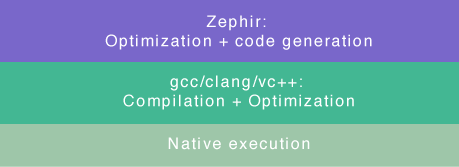
\includegraphics{scheme.png}
\end{figure}

In addition to the ones provided by Zephir, Over time, compilers have been implemented
and matured a number of optimizations that improve the performance of compiled applications:
\begin{itemize}
\item {} 
\href{http://gcc.gnu.org/onlinedocs/gcc-4.1.0/gcc/Optimize-Options.html}{GCC optimizations}

\item {} 
\href{http://llvm.org/docs/Passes.html}{LLVM passes}

\item {} 
\href{http://msdn.microsoft.com/en-us/library/k1ack8f1.aspx}{Visual C/C++ optimizations}

\end{itemize}


\subsection{Conclusion}
\label{motivation:conclusion}
Zephir was not created to replace PHP or C, instead of this, we think it is a complement to them,
allowing developers to venture into code compilation and static typing.
Zephir is precisely an attempt to join good things from the C and PHP worlds, looking for oportunities
to make their applications faster.


\section{Introducing Zephir}
\label{intro::doc}\label{intro:introducing-zephir}
Zephir is a language that addresses the major needs of a PHP developer trying to write and compile code that
can be executed by PHP. It is a dynamically/statically typed, some of its features can be familiar to
PHP developers.

The name Zephir is a contraction of the words Zend Engine/PHP/Intermediate. While this suggests that the
pronunciation should be zephyr, the creators of Zephir actually pronounce it \href{http://translate.google.com/\#en/en/zaefire}{zaefire}.


\subsection{Hello World!}
\label{intro:hello-world}
Every language has its own ``Hello World!'' sample, in Zephir this introductory example showcase some important
features of this language.

Code in Zephir must be placed in classes, Zephir is intended to create object-oriented libraries/frameworks,
so code out of a class is not allowed. Also a namespace is required:

\begin{Verbatim}[commandchars=\\\{\}]
\PYG{n+nx}{namespace} \PYG{n+nx}{Test}\PYG{p}{;}

\PYG{c+cm}{/**}
\PYG{c+cm}{ * This is a sample class}
\PYG{c+cm}{ */}
\PYG{k+kr}{class} \PYG{n+nx}{Hello}
\PYG{p}{\PYGZob{}}
    \PYG{c+cm}{/**}
\PYG{c+cm}{     * This is a sample method}
\PYG{c+cm}{     */}
    \PYG{k+kr}{public} \PYG{k+kd}{function} \PYG{n+nx}{say}\PYG{p}{(}\PYG{p}{)}
    \PYG{p}{\PYGZob{}}
        \PYG{n+nx}{echo} \PYG{l+s+s2}{"Hello World!"}\PYG{p}{;}
    \PYG{p}{\PYGZcb{}}
\PYG{p}{\PYGZcb{}}
\end{Verbatim}

Once this class is compiled it produce the following code that is transparently compiled by gcc/clang/vc++:

\begin{Verbatim}[commandchars=\\\{\}]
\PYG{c+cp}{\PYGZsh{}}\PYG{c+cp}{ifdef HAVE\PYGZus{}CONFIG\PYGZus{}H}
\PYG{c+cp}{\PYGZsh{}}\PYG{c+cp}{include "config.h"}
\PYG{c+cp}{\PYGZsh{}}\PYG{c+cp}{endif}

\PYG{c+cp}{\PYGZsh{}}\PYG{c+cp}{include "php.h"}
\PYG{c+cp}{\PYGZsh{}}\PYG{c+cp}{include "php\PYGZus{}test.h"}
\PYG{c+cp}{\PYGZsh{}}\PYG{c+cp}{include "test.h"}

\PYG{c+cp}{\PYGZsh{}}\PYG{c+cp}{include "kernel}\PYG{c+cp}{/}\PYG{c+cp}{main.h"}

\PYG{c+cm}{/**}
\PYG{c+cm}{ * This is a sample class}
\PYG{c+cm}{ */}
\PYG{n}{ZEPHIR\PYGZus{}INIT\PYGZus{}CLASS}\PYG{p}{(}\PYG{n}{Test\PYGZus{}Hello}\PYG{p}{)} \PYG{p}{\PYGZob{}}
    \PYG{n}{ZEPHIR\PYGZus{}REGISTER\PYGZus{}CLASS}\PYG{p}{(}\PYG{n}{Test}\PYG{p}{,} \PYG{n}{Hello}\PYG{p}{,} \PYG{n}{hello}\PYG{p}{,} \PYG{n}{test\PYGZus{}hello\PYGZus{}method\PYGZus{}entry}\PYG{p}{,} \PYG{l+m+mi}{0}\PYG{p}{)}\PYG{p}{;}
    \PYG{k}{return} \PYG{n}{SUCCESS}\PYG{p}{;}
\PYG{p}{\PYGZcb{}}

\PYG{c+cm}{/**}
\PYG{c+cm}{ * This is a sample method}
\PYG{c+cm}{ */}
\PYG{n}{PHP\PYGZus{}METHOD}\PYG{p}{(}\PYG{n}{Test\PYGZus{}Hello}\PYG{p}{,} \PYG{n}{say}\PYG{p}{)} \PYG{p}{\PYGZob{}}
    \PYG{n}{php\PYGZus{}printf}\PYG{p}{(}\PYG{l+s}{"}\PYG{l+s}{\PYGZpc{}s}\PYG{l+s}{"}\PYG{p}{,} \PYG{l+s}{"}\PYG{l+s}{Hello World!}\PYG{l+s}{"}\PYG{p}{)}\PYG{p}{;}
\PYG{p}{\PYGZcb{}}
\end{Verbatim}

Actually, it is not expected that a developer that uses Zephir must know or even understand C,
however if you have any experience with compilers, php internals or the C language itself,
it would provide a more clear sceneario to the developer when working with Zephir.


\subsection{A Taste of Zephir}
\label{intro:a-taste-of-zephir}
In the following examples, we’ll describe just enough of the details so you understand what’s going on.
The goal is to give you a sense of what programming in Zephir is like. We’ll explore the details of the
features in subsequent chapters.

The following example is very simple, it implements a class and a method with an small program that checks
the types of an array

Let’s examine the code in detail, so we can begin to learn Zephir syntax.
There are a lot of details in just a few lines of code! We’ll explain the general ideas here:

\begin{Verbatim}[commandchars=\\\{\}]
\PYG{n+nx}{namespace} \PYG{n+nx}{Test}\PYG{p}{;}

\PYG{c+cm}{/**}
\PYG{c+cm}{ * MyTest (test/mytest.zep)}
\PYG{c+cm}{ */}
\PYG{k+kr}{class} \PYG{n+nx}{MyTest}
\PYG{p}{\PYGZob{}}
    \PYG{k+kr}{public} \PYG{k+kd}{function} \PYG{n+nx}{someMethod}\PYG{p}{(}\PYG{p}{)}
    \PYG{p}{\PYGZob{}}
        \PYG{c+cm}{/* Variables must be declared */}
        \PYG{k+kd}{var} \PYG{n+nx}{myArray}\PYG{p}{;}
        \PYG{k+kr}{int} \PYG{n+nx}{i} \PYG{o}{=} \PYG{l+m+mi}{0}\PYG{p}{,} \PYG{n+nx}{length}\PYG{p}{;}

        \PYG{c+cm}{/* Create an array */}
        \PYG{n+nx}{let} \PYG{n+nx}{myArray} \PYG{o}{=} \PYG{p}{[}\PYG{l+s+s2}{"hello"}\PYG{p}{,} \PYG{l+m+mi}{0}\PYG{p}{,} \PYG{l+m+mf}{100.25}\PYG{p}{,} \PYG{k+kc}{false}\PYG{p}{,} \PYG{k+kc}{null}\PYG{p}{]}\PYG{p}{;}

        \PYG{c+cm}{/* Count the array into a 'int' variable */}
        \PYG{n+nx}{let} \PYG{n+nx}{length} \PYG{o}{=} \PYG{n+nx}{count}\PYG{p}{(}\PYG{n+nx}{myArray}\PYG{p}{)}\PYG{p}{;}

        \PYG{c+cm}{/* Print value types */}
        \PYG{k}{while} \PYG{n+nx}{i} \PYG{o}{\textless{}} \PYG{n+nx}{length} \PYG{p}{\PYGZob{}}
            \PYG{n+nx}{echo} \PYG{k}{typeof} \PYG{n+nx}{myArray}\PYG{p}{[}\PYG{n+nx}{i}\PYG{p}{]}\PYG{p}{,} \PYG{l+s+s2}{"\PYGZbs{}n"}\PYG{p}{;}
            \PYG{n+nx}{let} \PYG{n+nx}{i}\PYG{o}{++}\PYG{p}{;}
        \PYG{p}{\PYGZcb{}}

        \PYG{k}{return} \PYG{n+nx}{myArray}\PYG{p}{;}
    \PYG{p}{\PYGZcb{}}
\PYG{p}{\PYGZcb{}}
\end{Verbatim}

In the method, the first lines use the `var' and `int' keywords are used to declare a variables in a local scope.
Every variable used in a method must be declared with its respective type. This declaration is not optional,
it helps the compiler to report you about mistyped variables or about the use of variables out of their scope
which usually ends in runtime errors.

Dynamic variables are declared with the keyword `var'. These variables can be assigned and reassigned
to different types. On the other hand, we have `i' and `length' integer static typed variables
that can only have values of this type in the entire program execution.

In contrast with PHP you are not required to put a dollar sign (\$) in front of variable names.

Zephir follows the same comment conventions as Java, C\#, C++, etc.
A //comment goes to the end of a line, while a /* comment */ can cross line boundaries.

Variables are by default inmutable, this means that Zephir expects that most variables stay
unchanged. Variables that maintain their initial value can be optimized down by the compiler to static constants.
When the value of a variable needs to be changed, the keyword `let' must be used:

\begin{Verbatim}[commandchars=\\\{\}]
\PYG{c+cm}{/* Create an array */}
\PYG{n+nx}{let} \PYG{n+nx}{myArray} \PYG{o}{=} \PYG{p}{[}\PYG{l+s+s2}{"hello"}\PYG{p}{,} \PYG{l+m+mi}{0}\PYG{p}{,} \PYG{l+m+mf}{100.25}\PYG{p}{,} \PYG{k+kc}{false}\PYG{p}{,} \PYG{k+kc}{null}\PYG{p}{]}\PYG{p}{;}
\end{Verbatim}

By default, arrays are dynamic like in PHP, they may contain values of different types.
Functions from the PHP userland can be called in Zephir code, in the example the function `count'
was called, the compiler can performs optimizations like avoid this call because it already knows the size of
the array:

\begin{Verbatim}[commandchars=\\\{\}]
\PYG{c+cm}{/* Count the array into a 'int' variable */}
\PYG{n+nx}{let} \PYG{n+nx}{length} \PYG{o}{=} \PYG{n+nx}{count}\PYG{p}{(}\PYG{n+nx}{myArray}\PYG{p}{)}\PYG{p}{;}
\end{Verbatim}

Parentheses in control flow statements are optional, you can also use them if you feel more confortable.

\begin{Verbatim}[commandchars=\\\{\}]
\PYG{k}{while} \PYG{n+nx}{i} \PYG{o}{\textless{}} \PYG{n+nx}{length} \PYG{p}{\PYGZob{}}
    \PYG{n+nx}{echo} \PYG{k}{typeof} \PYG{n+nx}{myArray}\PYG{p}{[}\PYG{n+nx}{i}\PYG{p}{]}\PYG{p}{,} \PYG{l+s+s2}{"\PYGZbs{}n"}\PYG{p}{;}
    \PYG{n+nx}{let} \PYG{n+nx}{i}\PYG{o}{++}\PYG{p}{;}
\PYG{p}{\PYGZcb{}}
\end{Verbatim}

PHP only works with dynamic variables, methods always return dynamic variables, this means that if a
static typed variable is returned, in the PHP side, you will get a dynamic variable that can be used
in PHP code. Note that memory is automatically managed by the compiler, so you don't need to allocate or free
memory like in C, working in a similar way than PHP.


\section{Tutorial}
\label{tutorial:zaefire}\label{tutorial::doc}\label{tutorial:tutorial}
Zephir and this book are intended for PHP developers which wants to create C-extensions with a lower
complexity.

We assume that you are experienced in one or more other programming languages. We draw parallels to features
in PHP, C, Javascript, and other languages. If you know any of these languages, we’ll point out
similar features in Zephir, as well as many features that are new or different.


\section{Basic Syntax}
\label{language::doc}\label{language:basic-syntax}
In this chapter, we’ll discuss the organization of files and namespaces, variable declarations,
miscellaneous syntax conventions, and a few other concepts.


\subsection{Organizing Code in Files and Namespaces}
\label{language:organizing-code-in-files-and-namespaces}
In PHP, you can place code in any file without a specific structure. In Zephir every file must contain
a class (and just one class). Every class must have a namespace and the directory structure must match
the names of classes and namespaces used.

For example given the following structure, the classes in each file must be:

\begin{Verbatim}[commandchars=\\\{\}]
mylibrary/
        router/
                exception.zep \PYG{c}{\PYGZsh{} MyLibrary\PYGZbs{}Router\PYGZbs{}Exception}
        router.zep \PYG{c}{\PYGZsh{} MyLibrary\PYGZbs{}Router}
\end{Verbatim}

Class in mylibrary/router.zep:

\begin{Verbatim}[commandchars=\\\{\}]
\PYG{n+nx}{namespace} \PYG{n+nx}{MyLibrary}\PYG{p}{;}

\PYG{k+kr}{class} \PYG{n+nx}{Router}
\PYG{p}{\PYGZob{}}

\PYG{p}{\PYGZcb{}}
\end{Verbatim}

Class in mylibrary/router/exception.zep:

\begin{Verbatim}[commandchars=\\\{\}]
\PYG{x}{namespace MyLibrary\PYGZbs{}Router;}

\PYG{x}{class Router extends Exception}
\PYG{x}{\PYGZob{}}

\PYG{x}{\PYGZcb{}}
\end{Verbatim}

Zephir will raise a compiler exception if a file or class is not located at the expected file or vice versa.


\subsection{Instruction separation}
\label{language:instruction-separation}
You may have already noticed that there were very few semicolons in the code examples in the previous chapter.
You can use semicolons to separate statements and expressions, as in Java, C/C++, PHP, and similar languages:

\begin{Verbatim}[commandchars=\\\{\}]
\PYG{n+nx}{myObject}\PYG{o}{-}\PYG{o}{\textgreater{}}\PYG{n+nx}{myMethod}\PYG{p}{(}\PYG{l+m+mi}{1}\PYG{p}{,} \PYG{l+m+mi}{2}\PYG{p}{,} \PYG{l+m+mi}{3}\PYG{p}{)}\PYG{p}{;} \PYG{n+nx}{echo} \PYG{l+s+s2}{"world"}\PYG{p}{;}
\end{Verbatim}


\subsection{Comments}
\label{language:comments}
Zephir supports `C'/'C++' comments, these are one line comments with // and multi line comments with /* ... */:

\begin{Verbatim}[commandchars=\\\{\}]
\PYG{c+c1}{// this is one line comment}

\PYG{c+cm}{/**}
\PYG{c+cm}{ * multi-line comment}
\PYG{c+cm}{ */}
\end{Verbatim}

In most languages comments are simply text ignored by the compiler/interpreter. In Zephir,
multi-line comments are also used as docblocks and they're exported to the generated code,
so they're part of the language!.

The compiler would throw an exception if a docblock is not located where is expected.


\subsection{Variable Declarations}
\label{language:variable-declarations}
In Zephir, all variables used in a given scope must be declared, this process gives important information
to the compiler to perform optimizations and validations. Variables must be unique identifiers and they cannot be
reserved words.

\begin{Verbatim}[commandchars=\\\{\}]
\PYG{c+c1}{//Declaring variables for the same type in the same instruction}
\PYG{k+kd}{var} \PYG{n+nx}{a}\PYG{p}{,} \PYG{n+nx}{b} \PYG{n+nx}{c}\PYG{p}{;}

\PYG{c+c1}{//Declaring each variable in different lines}
\PYG{k+kd}{var} \PYG{n+nx}{a}\PYG{p}{;}
\PYG{k+kd}{var} \PYG{n+nx}{b}\PYG{p}{;}
\PYG{k+kd}{var} \PYG{n+nx}{c}\PYG{p}{;}
\end{Verbatim}

Variables can optionally have an initial compatible default value, you can assign a new value to a variable
as often as you want:

\begin{Verbatim}[commandchars=\\\{\}]
\PYG{c+c1}{//Declaring variables with default values}
\PYG{k+kd}{var} \PYG{n+nx}{a} \PYG{o}{=} \PYG{l+s+s2}{"hello"}\PYG{p}{,} \PYG{n+nx}{b} \PYG{o}{=} \PYG{l+m+mi}{0}\PYG{p}{,} \PYG{n+nx}{c} \PYG{o}{=} \PYG{l+m+mf}{1.0}\PYG{p}{;}
\PYG{k+kr}{int} \PYG{n+nx}{d} \PYG{o}{=} \PYG{l+m+mi}{50}\PYG{p}{;} \PYG{n+nx}{bool} \PYG{n+nx}{some} \PYG{o}{=} \PYG{k+kc}{true}\PYG{p}{;}
\end{Verbatim}

Variable names are case-sensitive, the following variables are different:

\begin{Verbatim}[commandchars=\\\{\}]
\PYG{c+c1}{//Different variables}
\PYG{k+kd}{var} \PYG{n+nx}{somevalue}\PYG{p}{,} \PYG{n+nx}{someValue}\PYG{p}{,} \PYG{n+nx}{SomeValue}\PYG{p}{;}
\end{Verbatim}


\subsection{Variable Scope}
\label{language:variable-scope}
All variables declared are locally scoped to the method where they were declared:

\begin{Verbatim}[commandchars=\\\{\}]
\PYG{n+nx}{namespace} \PYG{n+nx}{Test}\PYG{p}{;}

\PYG{k+kr}{class} \PYG{n+nx}{MyClass}
\PYG{p}{\PYGZob{}}

    \PYG{k+kr}{public} \PYG{k+kd}{function} \PYG{n+nx}{someMethod1}\PYG{p}{(}\PYG{p}{)}
    \PYG{p}{\PYGZob{}}
        \PYG{k+kr}{int} \PYG{n+nx}{a} \PYG{o}{=} \PYG{l+m+mi}{1}\PYG{p}{,} \PYG{n+nx}{b} \PYG{o}{=} \PYG{l+m+mi}{2}\PYG{p}{;}
        \PYG{k}{return} \PYG{n+nx}{a} \PYG{o}{+} \PYG{n+nx}{b}\PYG{p}{;}
    \PYG{p}{\PYGZcb{}}

    \PYG{k+kr}{public} \PYG{k+kd}{function} \PYG{n+nx}{someMethod2}\PYG{p}{(}\PYG{p}{)}
    \PYG{p}{\PYGZob{}}
        \PYG{k+kr}{int} \PYG{n+nx}{a} \PYG{o}{=} \PYG{l+m+mi}{3}\PYG{p}{,} \PYG{n+nx}{b} \PYG{o}{=} \PYG{l+m+mi}{4}\PYG{p}{;}
        \PYG{k}{return} \PYG{n+nx}{a} \PYG{o}{+} \PYG{n+nx}{b}\PYG{p}{;}
    \PYG{p}{\PYGZcb{}}

\PYG{p}{\PYGZcb{}}
\end{Verbatim}


\subsection{Super Globals}
\label{language:super-globals}
Zephir doesn't support global variables, accessing global variables from the PHP userland is not allowed.
However, you can access the PHP's super-globals as follows:

\begin{Verbatim}[commandchars=\\\{\}]
\PYG{c+c1}{//Getting a value from \PYGZus{}POST}
\PYG{n+nx}{let} \PYG{n+nx}{price} \PYG{o}{=} \PYG{n+nx}{\PYGZus{}POST}\PYG{p}{[}\PYG{l+s+s1}{'price'}\PYG{p}{]}\PYG{p}{;}

\PYG{c+c1}{//Read a value from \PYGZus{}SERVER}
\PYG{n+nx}{let} \PYG{n+nx}{requestMethod} \PYG{o}{=} \PYG{n+nx}{\PYGZus{}SERVER}\PYG{p}{[}\PYG{l+s+s1}{'REQUEST\PYGZus{}METHOD'}\PYG{p}{]}\PYG{p}{;}
\end{Verbatim}


\subsection{Local Symbol Table}
\label{language:local-symbol-table}
Every method or context in PHP has a symbol table that allows to write variables in a very dynamic
way:

\begin{Verbatim}[commandchars=\\\{\}]
\PYG{c+cp}{\textless{}?php}

\PYG{n+nv}{\PYGZdl{}b} \PYG{o}{=} \PYG{l+m+mi}{100}\PYG{p}{;}
\PYG{n+nv}{\PYGZdl{}a} \PYG{o}{=} \PYG{l+s+s2}{"}\PYG{l+s+s2}{b}\PYG{l+s+s2}{"}\PYG{p}{;}
\PYG{k}{echo} \PYG{n+nv}{\PYGZdl{}\PYGZdl{}a}\PYG{p}{;} \PYG{c+c1}{// prints 100}
\end{Verbatim}

Zephir does not implement this feature since all variables are compiled down to low level variables,
and there is no way to know which variables exist in a specific context.


\section{Types}
\label{types::doc}\label{types:types}
Zephir is both dynamic and static typed. In this chapter we highlight the supported types and
its behavior:


\subsection{Dynamic Type}
\label{types:dynamic-type}
Dynamic variables are exactly like the ones in PHP, they can be assigned and reassigned to
different types without restriction.

A dynamic variable must be declared with the keyword `var', the behavior is nearly the same as in PHP:

\begin{Verbatim}[commandchars=\\\{\}]
\PYG{k+kd}{var} \PYG{n+nx}{a}\PYG{p}{,} \PYG{n+nx}{b}\PYG{p}{,} \PYG{n+nx}{c}\PYG{p}{;}

\PYG{c+c1}{// Initialize variables}
\PYG{n+nx}{let} \PYG{n+nx}{a} \PYG{o}{=} \PYG{l+s+s2}{"hello"}\PYG{p}{,} \PYG{n+nx}{b} \PYG{o}{=} \PYG{k+kc}{false}\PYG{p}{;}

\PYG{c+c1}{// Change their values}
\PYG{n+nx}{let} \PYG{n+nx}{a} \PYG{o}{=} \PYG{l+m+mi}{10}\PYG{p}{,} \PYG{n+nx}{b} \PYG{o}{=} \PYG{l+s+s2}{"140"}\PYG{p}{;}

\PYG{c+c1}{// Perform operations between them}
\PYG{n+nx}{let} \PYG{n+nx}{c} \PYG{o}{=} \PYG{n+nx}{a} \PYG{o}{+} \PYG{n+nx}{b}\PYG{p}{;}
\end{Verbatim}

They can have eight types:

\begin{tabulary}{\linewidth}{|L|L|}
\hline

Type
 & 
Description
\\\hline

boolean
 & 
A boolean expresses a truth value. It can be either `true' or `false'.
\\\hline

integer
 & 
Integer numbers. The size of an integer is platform-dependent.
\\\hline

float/double
 & 
Floating point numbers. The size of a float is platform-dependent.
\\\hline

string
 & 
A string is series of characters, where a character is the same as a byte.
\\\hline

array
 & 
An array is an ordered map. A map is a type that associates values to keys
\\\hline

object
 & 
Object abstraction like in PHP
\\\hline

resource
 & 
A resource holds a reference to an external resource
\\\hline

null
 & 
The special NULL value represents a variable with no value
\\\hline
\end{tabulary}


Check more info about these types in the \href{http://www.php.net/manual/en/language.types.php}{PHP manual}


\subsubsection{Boolean}
\label{types:boolean}
A boolean expresses a truth value. It can be either `true' or `false':

\begin{Verbatim}[commandchars=\\\{\}]
\PYG{k+kd}{var} \PYG{n+nx}{a} \PYG{o}{=} \PYG{k+kc}{false}\PYG{p}{,} \PYG{n+nx}{b} \PYG{o}{=} \PYG{k+kc}{true}\PYG{p}{;}
\end{Verbatim}


\subsubsection{Integer}
\label{types:integer}
Integer numbers. The size of an integer is platform-dependent, although a maximum value of about two
billion is the usual value (that's 32 bits signed). 64-bit platforms usually have a maximum value of about 9E18.
PHP does not support unsigned integers so Zephir has this restriction too:

\begin{Verbatim}[commandchars=\\\{\}]
\PYG{k+kd}{var} \PYG{n+nx}{a} \PYG{o}{=} \PYG{l+m+mi}{5}\PYG{p}{,} \PYG{n+nx}{b} \PYG{o}{=} \PYG{l+m+mi}{10050}\PYG{p}{;}
\end{Verbatim}


\subsubsection{Integer overflow}
\label{types:integer-overflow}
Contrary to PHP, Zephir does not automatically checks for integer overflows, like in C if you are
doing operations that may return a big number you can use types such as `unsigned long' or `float'
to store them:

\begin{Verbatim}[commandchars=\\\{\}]
\PYG{n+nx}{unsigned} \PYG{k+kr}{long} \PYG{n+nx}{my\PYGZus{}number} \PYG{o}{=} \PYG{l+m+mi}{2147483648}\PYG{p}{;}
\end{Verbatim}


\subsubsection{Float/Double}
\label{types:float-double}
Floating-point numbers (also known as ``floats'', ``doubles'', or ``real numbers'').
Floating-point literals are expressions with zero or more digits, followed by a period (.),
followed by zero or more digits. The size of a float is
platform-dependent, although a maximum of \textasciitilde{}1.8e308 with a
precision of roughly 14 decimal digits is a common value (the 64 bit IEEE format).

\begin{Verbatim}[commandchars=\\\{\}]
\PYG{k+kd}{var} \PYG{n+nx}{number} \PYG{o}{=} \PYG{l+m+mf}{5.0}\PYG{p}{,} \PYG{n+nx}{b} \PYG{o}{=} \PYG{l+m+mf}{0.014}\PYG{p}{;}
\end{Verbatim}

Floating point numbers have limited precision. Although it depends on the system,
as PHP, Zephir uses the IEEE 754 double precision format, which will give a maximum
relative error due to rounding in the order of 1.11e-16.


\subsubsection{String}
\label{types:string}
A string is series of characters, where a character is the same as a byte. As PHP, Zephir only supports
a 256-character set, and hence does not offer native Unicode support.

\begin{Verbatim}[commandchars=\\\{\}]
\PYG{k+kd}{var} \PYG{n+nx}{today} \PYG{o}{=} \PYG{l+s+s2}{"friday"}\PYG{p}{;}
\end{Verbatim}

In Zephir, string literals can only be specified using double quotes (like in C), single quotes are reserved
for chars.

The following escape sequences are supported in strings:

\begin{tabulary}{\linewidth}{|L|L|}
\hline

Sequence
 & 
Description
\\\hline

\textbackslash{}t
 & 
Horizontal tab
\\\hline

\textbackslash{}n
 & 
Line feed
\\\hline

\textbackslash{}r
 & 
Carriage return
\\\hline

\textbackslash{} \textbackslash{}
 & 
Backslash
\\\hline

\textbackslash{}''
 & 
double-quote
\\\hline
\end{tabulary}


\begin{Verbatim}[commandchars=\\\{\}]
\PYG{k+kd}{var} \PYG{n+nx}{today} \PYG{o}{=} \PYG{l+s+s2}{"\PYGZbs{}tfriday\PYGZbs{}n\PYGZbs{}r"}\PYG{p}{,}
    \PYG{n+nx}{tomorrow} \PYG{o}{=} \PYG{l+s+s2}{"\PYGZbs{}tsaturday"}\PYG{p}{;}
\end{Verbatim}

In Zephir, strings don't support variable parsing like in PHP, you can use concatenation instead:

\begin{Verbatim}[commandchars=\\\{\}]
\PYG{k+kd}{var} \PYG{n+nx}{name} \PYG{o}{=} \PYG{l+s+s2}{"peter"}\PYG{p}{;}

\PYG{n+nx}{echo} \PYG{l+s+s2}{"hello: "} \PYG{p}{.} \PYG{n+nx}{name}\PYG{p}{;}
\end{Verbatim}


\subsubsection{Arrays}
\label{types:arrays}
The array implementation in Zephir is basically the same as in PHP: Ordered maps optimized for
several different uses; it can be treated as an array, list (vector), hash table (an implementation of a map),
dictionary, collection, stack, queue, and probably more. As array values can be other arrays, trees and
multidimensional arrays are also possible.

The syntax to define arrays is slightly different than in PHP:

\begin{Verbatim}[commandchars=\\\{\}]
\PYG{c+c1}{//Square braces must be used to define arrays}
\PYG{n+nx}{let} \PYG{n+nx}{myArray} \PYG{o}{=} \PYG{p}{[}\PYG{l+m+mi}{1}\PYG{p}{,} \PYG{l+m+mi}{2}\PYG{p}{,} \PYG{l+m+mi}{3}\PYG{p}{]}\PYG{p}{;}

\PYG{c+c1}{//Double colon must be used to define hashes' keys}
\PYG{n+nx}{let} \PYG{n+nx}{myHash} \PYG{o}{=} \PYG{p}{[}\PYG{l+s+s2}{"first"}\PYG{o}{:} \PYG{l+m+mi}{1}\PYG{p}{,} \PYG{l+s+s2}{"second"}\PYG{o}{:} \PYG{l+m+mi}{2}\PYG{p}{,} \PYG{l+s+s2}{"third"}\PYG{o}{:} \PYG{l+m+mi}{3}\PYG{p}{]}\PYG{p}{;}
\end{Verbatim}

Only long and string values can be used as keys:

\begin{Verbatim}[commandchars=\\\{\}]
\PYG{n+nx}{let} \PYG{n+nx}{myHash} \PYG{o}{=} \PYG{p}{[}\PYG{l+m+mi}{0}\PYG{o}{:} \PYG{l+s+s2}{"first"}\PYG{p}{,} \PYG{l+m+mi}{1}\PYG{o}{:} \PYG{k+kc}{true}\PYG{p}{,} \PYG{l+m+mi}{2}\PYG{o}{:} \PYG{k+kc}{null}\PYG{p}{]}\PYG{p}{;}
\PYG{n+nx}{let} \PYG{n+nx}{myHash} \PYG{o}{=} \PYG{p}{[}\PYG{l+s+s2}{"first"}\PYG{o}{:} \PYG{l+m+mf}{7.0}\PYG{p}{,} \PYG{l+s+s2}{"second"}\PYG{o}{:} \PYG{l+s+s2}{"some string"}\PYG{p}{,} \PYG{l+s+s2}{"third"}\PYG{o}{:} \PYG{k+kc}{false}\PYG{p}{]}\PYG{p}{;}
\end{Verbatim}


\subsubsection{Objects}
\label{types:objects}
Zephir allows to instantiate, manipulate, call methods, read class constants, etc from PHP objects:

\begin{Verbatim}[commandchars=\\\{\}]
\PYG{n+nx}{let} \PYG{n+nx}{myObject} \PYG{o}{=} \PYG{k}{new} \PYG{n+nx}{stdClass}\PYG{p}{(}\PYG{p}{)}\PYG{p}{,}
    \PYG{n+nx}{myObject}\PYG{o}{-}\PYG{o}{\textgreater{}}\PYG{n+nx}{someProperty} \PYG{o}{=} \PYG{l+s+s2}{"my value"}\PYG{p}{;}
\end{Verbatim}


\subsection{Static Types}
\label{types:static-types}
Static typing allows the developer to declare and use some variable types available in C.
Variables can't change their type once they're declared as dynamic types. However, they allow
the compiler to do a better optimization job. The following types are supported:

\begin{tabulary}{\linewidth}{|L|L|}
\hline

Type
 & 
Description
\\\hline

boolean
 & 
A boolean expresses a truth value. It can be either `true' or `false'.
\\\hline

integer
 & 
Signed integers. At least 16 bits in size.
\\\hline

unsigned integer
 & 
Unsigned integers. At least 16 bits in size.
\\\hline

char
 & 
Smallest addressable unit of the machine that can contain basic character set.
\\\hline

unsigned char
 & 
Same size as char, but guaranteed to be unsigned.
\\\hline

long
 & 
Long signed integer type. At least 32 bits in size.
\\\hline

unsigned long
 & 
Same as long, but unsigned.
\\\hline

float/double
 & 
Double precision floating-point type. The size is platform-dependent.
\\\hline

string
 & 
A string is series of characters, where a character is the same as a byte.
\\\hline
\end{tabulary}



\subsubsection{Boolean}
\label{types:id1}
A boolean expresses a truth value. It can be either `true' or `false'. Contrary to the dynamic behavior
static boolean types remain boolean (true or false) no mater what value is assigned to them:

\begin{Verbatim}[commandchars=\\\{\}]
\PYG{k+kr}{boolean} \PYG{n+nx}{a}\PYG{p}{;}

\PYG{n+nx}{let} \PYG{n+nx}{a} \PYG{o}{=} \PYG{k+kc}{true}\PYG{p}{,}
    \PYG{n+nx}{a} \PYG{o}{=} \PYG{l+m+mi}{100}\PYG{p}{,} \PYG{c+c1}{// automatically casted to true}
    \PYG{n+nx}{a} \PYG{o}{=} \PYG{k+kc}{null}\PYG{p}{,} \PYG{c+c1}{// automatically casted to false}
    \PYG{n+nx}{a} \PYG{o}{=} \PYG{l+s+s2}{"hello"}\PYG{p}{;} \PYG{c+c1}{// throws a compiler exception}
\end{Verbatim}


\subsubsection{Integer/Unsigned Integer}
\label{types:integer-unsigned-integer}
Integer values are like the integer member in dynamic values. Values assigned to integer variables
remain integer:

\begin{Verbatim}[commandchars=\\\{\}]
\PYG{k+kr}{int} \PYG{n+nx}{a}\PYG{p}{;}

\PYG{n+nx}{let} \PYG{n+nx}{a} \PYG{o}{=} \PYG{l+m+mi}{50}\PYG{p}{,}
    \PYG{n+nx}{a} \PYG{o}{=} \PYG{o}{-}\PYG{l+m+mi}{70}\PYG{p}{,}
    \PYG{n+nx}{a} \PYG{o}{=} \PYG{l+m+mf}{100.25}\PYG{p}{,} \PYG{c+c1}{// automatically casted to 100}
    \PYG{n+nx}{a} \PYG{o}{=} \PYG{k+kc}{null}\PYG{p}{,} \PYG{c+c1}{// automatically casted to 0}
    \PYG{n+nx}{a} \PYG{o}{=} \PYG{k+kc}{false}\PYG{p}{,} \PYG{c+c1}{// automatically casted to 0}
    \PYG{n+nx}{a} \PYG{o}{=} \PYG{l+s+s2}{"hello"}\PYG{p}{;} \PYG{c+c1}{// throws a compiler exception}
\end{Verbatim}

Unsigned integers are like integers but they don't have sign, this means you can't store
negative numbers in these sort of variables:

\begin{Verbatim}[commandchars=\\\{\}]
\PYG{n+nx}{let} \PYG{n+nx}{a} \PYG{o}{=} \PYG{l+m+mi}{50}\PYG{p}{,}
    \PYG{n+nx}{a} \PYG{o}{=} \PYG{o}{-}\PYG{l+m+mi}{70}\PYG{p}{,} \PYG{c+c1}{// automatically casted to 70}
    \PYG{n+nx}{a} \PYG{o}{=} \PYG{l+m+mf}{100.25}\PYG{p}{,} \PYG{c+c1}{// automatically casted to 100}
    \PYG{n+nx}{a} \PYG{o}{=} \PYG{k+kc}{null}\PYG{p}{,} \PYG{c+c1}{// automatically casted to 0}
    \PYG{n+nx}{a} \PYG{o}{=} \PYG{k+kc}{false}\PYG{p}{,} \PYG{c+c1}{// automatically casted to 0}
    \PYG{n+nx}{a} \PYG{o}{=} \PYG{l+s+s2}{"hello"}\PYG{p}{;} \PYG{c+c1}{// throws a compiler exception}
\end{Verbatim}

Unsigned integers are twice bigger than standard integers, assign unsigned integers to integers
may represent loss of data:

\begin{Verbatim}[commandchars=\\\{\}]
\PYG{n+nx}{uint} \PYG{n+nx}{a}\PYG{p}{,} \PYG{k+kr}{int} \PYG{n+nx}{b}\PYG{p}{;}

\PYG{n+nx}{let} \PYG{n+nx}{a} \PYG{o}{=} \PYG{l+m+mi}{2147483648}\PYG{p}{,}
    \PYG{n+nx}{b} \PYG{o}{=} \PYG{n+nx}{a}\PYG{p}{,} \PYG{c+c1}{// possible loss of data}
\end{Verbatim}


\subsubsection{Long/Unsigned Long}
\label{types:long-unsigned-long}
Long variables are twice bigger than integer variables, thus they can store bigger numbers,
As integers values assigned to long variables are automatically casted to this type:

\begin{Verbatim}[commandchars=\\\{\}]
\PYG{k+kr}{long} \PYG{n+nx}{a}\PYG{p}{;}

\PYG{n+nx}{let} \PYG{n+nx}{a} \PYG{o}{=} \PYG{l+m+mi}{50}\PYG{p}{,}
    \PYG{n+nx}{a} \PYG{o}{=} \PYG{o}{-}\PYG{l+m+mi}{70}\PYG{p}{,}
    \PYG{n+nx}{a} \PYG{o}{=} \PYG{l+m+mf}{100.25}\PYG{p}{,} \PYG{c+c1}{// automatically casted to 100}
    \PYG{n+nx}{a} \PYG{o}{=} \PYG{k+kc}{null}\PYG{p}{,} \PYG{c+c1}{// automatically casted to 0}
    \PYG{n+nx}{a} \PYG{o}{=} \PYG{k+kc}{false}\PYG{p}{,} \PYG{c+c1}{// automatically casted to 0}
    \PYG{n+nx}{a} \PYG{o}{=} \PYG{l+s+s2}{"hello"}\PYG{p}{;} \PYG{c+c1}{// throws a compiler exception}
\end{Verbatim}

Unsigned longs are like longs but they aren't signed, this means you can't store
negative numbers in these sort of variables:

\begin{Verbatim}[commandchars=\\\{\}]
\PYG{n+nx}{let} \PYG{n+nx}{a} \PYG{o}{=} \PYG{l+m+mi}{50}\PYG{p}{,}
    \PYG{n+nx}{a} \PYG{o}{=} \PYG{o}{-}\PYG{l+m+mi}{70}\PYG{p}{,} \PYG{c+c1}{// automatically casted to 70}
    \PYG{n+nx}{a} \PYG{o}{=} \PYG{l+m+mf}{100.25}\PYG{p}{,} \PYG{c+c1}{// automatically casted to 100}
    \PYG{n+nx}{a} \PYG{o}{=} \PYG{k+kc}{null}\PYG{p}{,} \PYG{c+c1}{// automatically casted to 0}
    \PYG{n+nx}{a} \PYG{o}{=} \PYG{k+kc}{false}\PYG{p}{,} \PYG{c+c1}{// automatically casted to 0}
    \PYG{n+nx}{a} \PYG{o}{=} \PYG{l+s+s2}{"hello"}\PYG{p}{;} \PYG{c+c1}{// throws a compiler exception}
\end{Verbatim}

Unsigned longs are twice bigger than standard longs, assign unsigned longs to longs
may represent loss of data:

\begin{Verbatim}[commandchars=\\\{\}]
\PYG{n+nx}{ulong} \PYG{n+nx}{a}\PYG{p}{,} \PYG{k+kr}{long} \PYG{n+nx}{b}\PYG{p}{;}

\PYG{n+nx}{let} \PYG{n+nx}{a} \PYG{o}{=} \PYG{l+m+mi}{4294967296}\PYG{p}{,}
    \PYG{n+nx}{b} \PYG{o}{=} \PYG{n+nx}{a}\PYG{p}{,} \PYG{c+c1}{// possible loss of data}
\end{Verbatim}


\subsubsection{Char/Unsigned Char}
\label{types:char-unsigned-char}
Char variables are the smallest addressable unit of the machine that can contain basic character set.
Every `char' variable represents every character in a string:

\begin{Verbatim}[commandchars=\\\{\}]
\PYG{k+kr}{char} \PYG{n+nx}{ch}\PYG{p}{,} \PYG{n+nx}{string} \PYG{n+nx}{name} \PYG{o}{=} \PYG{l+s+s2}{"peter"}\PYG{p}{;}

\PYG{n+nx}{let} \PYG{n+nx}{ch} \PYG{o}{=} \PYG{n+nx}{name}\PYG{p}{[}\PYG{l+m+mi}{2}\PYG{p}{]}\PYG{p}{;} \PYG{c+c1}{// stores 't'}
\end{Verbatim}


\section{Operators}
\label{operators:php-manual}\label{operators:operators}\label{operators::doc}
Zephir's set of operators are similar to the ones PHP and also inherits some of their behaviors.


\subsection{Arithmetic Operators}
\label{operators:arithmetic-operators}
The following operators are supported:

\begin{tabulary}{\linewidth}{|L|L|}
\hline

Operation
 & 
Example
\\\hline

Negation
 & 
-a
\\\hline

Addition
 & 
a + b
\\\hline

Substraction
 & 
a - b
\\\hline

Multiplication
 & 
a * b
\\\hline

Division
 & 
a / b
\\\hline

Modulus
 & 
a \% b
\\\hline
\end{tabulary}



\subsection{Comparison Operators}
\label{operators:comparison-operators}
Comparison operators depend on the type of variables compared, for example, if both
compared operands are dynamic variables the behavior is the same as in PHP:

\begin{tabulary}{\linewidth}{|L|L|L|}
\hline

a == b
 & 
Equal
 & 
TRUE if a is equal to b after type juggling.
\\\hline

a === b
 & 
Identical
 & 
TRUE if a is equal to b, and they are of the same type.
\\\hline

a != b
 & 
Not equal
 & 
TRUE if a is not equal to b after type juggling.
\\\hline

a \textless{}\textgreater{} b
 & 
Not equal
 & 
TRUE if a is not equal to b after type juggling.
\\\hline

a !== b
 & 
Not identical
 & 
TRUE if a is not equal to b, or they are not of the same type.
\\\hline

a \textless{} b
 & 
Less than
 & 
TRUE if a is strictly less than b.
\\\hline

a \textgreater{} b
 & 
Greater than
 & 
TRUE if a is strictly greater than b.
\\\hline

a \textless{}= b
 & 
Less than or equal to
 & 
TRUE if a is less than or equal to b.
\\\hline

a \textgreater{}= b
 & 
Greater than or equal to
 & 
TRUE if a is greater than or equal to b.
\\\hline
\end{tabulary}


Learn more about comparison of dynamic variables in the \href{http://www.php.net/manual/en/language.operators.comparison.php}{php manual}.


\section{Arrays}
\label{arrays:arrays}\label{arrays:php-manual}\label{arrays::doc}
Array manipulation in Zephir provides a way to use PHP \href{http://www.php.net/manual/en/language.types.array.php}{arrays}.
An array is an implementation of a \href{http://en.wikipedia.org/wiki/Hash\_table}{hash table}.


\subsection{Creating Arrays}
\label{arrays:creating-arrays}
An array is created enclosing their elements in square brackets:

\begin{Verbatim}[commandchars=\\\{\}]
\PYG{c+c1}{//Creating an empty array}
\PYG{n+nx}{let} \PYG{n+nx}{elements} \PYG{o}{=} \PYG{p}{[}\PYG{p}{]}\PYG{p}{;}

\PYG{c+c1}{//Creating an array with elements}
\PYG{n+nx}{let} \PYG{n+nx}{elements} \PYG{o}{=} \PYG{p}{[}\PYG{l+m+mi}{1}\PYG{p}{,} \PYG{l+m+mi}{3}\PYG{p}{,} \PYG{l+m+mi}{4}\PYG{p}{]}\PYG{p}{;}

\PYG{c+c1}{//Creating an array with elements of different types}
\PYG{n+nx}{let} \PYG{n+nx}{elements} \PYG{o}{=} \PYG{p}{[}\PYG{l+s+s2}{"first"}\PYG{p}{,} \PYG{l+m+mi}{2}\PYG{p}{,} \PYG{k+kc}{true}\PYG{p}{]}\PYG{p}{;}

\PYG{c+c1}{//A multidimensional array}
\PYG{n+nx}{let} \PYG{n+nx}{elements} \PYG{o}{=} \PYG{p}{[}\PYG{p}{[}\PYG{l+m+mi}{0}\PYG{p}{,} \PYG{l+m+mi}{1}\PYG{p}{]}\PYG{p}{,} \PYG{p}{[}\PYG{l+m+mi}{4}\PYG{p}{,} \PYG{l+m+mi}{5}\PYG{p}{]}\PYG{p}{,} \PYG{p}{[}\PYG{l+m+mi}{2}\PYG{p}{,} \PYG{l+m+mi}{3}\PYG{p}{]}\PYG{p}{]}\PYG{p}{;}
\end{Verbatim}

As PHP, hashes or dictionaries are supported:

\begin{Verbatim}[commandchars=\\\{\}]
\PYG{c+c1}{//Creating a hash with string keys}
\PYG{n+nx}{let} \PYG{n+nx}{elements} \PYG{o}{=} \PYG{p}{[}\PYG{l+s+s2}{"foo"}\PYG{o}{:} \PYG{l+s+s2}{"bar"}\PYG{p}{,} \PYG{l+s+s2}{"bar"}\PYG{o}{:} \PYG{l+s+s2}{"foo"}\PYG{p}{]}\PYG{p}{;}

\PYG{c+c1}{//Creating a hash with numeric keys}
\PYG{n+nx}{let} \PYG{n+nx}{elements} \PYG{o}{=} \PYG{p}{[}\PYG{l+m+mi}{4}\PYG{o}{:} \PYG{l+s+s2}{"bar"}\PYG{p}{,} \PYG{l+m+mi}{8}\PYG{o}{:} \PYG{l+s+s2}{"foo"}\PYG{p}{]}\PYG{p}{;}

\PYG{c+c1}{//Creating a hash with mixed string and numeric keys}
\PYG{n+nx}{let} \PYG{n+nx}{elements} \PYG{o}{=} \PYG{p}{[}\PYG{l+m+mi}{4}\PYG{o}{:} \PYG{l+s+s2}{"bar"}\PYG{p}{,} \PYG{l+s+s2}{"foo"}\PYG{o}{:} \PYG{l+m+mi}{8}\PYG{p}{]}\PYG{p}{;}
\end{Verbatim}


\subsection{Updating arrays}
\label{arrays:updating-arrays}
Arrays are updated in the same way as PHP using square brackets:

\begin{Verbatim}[commandchars=\\\{\}]
\PYG{c+c1}{//Updating an array with a string key}
\PYG{n+nx}{let} \PYG{n+nx}{elements}\PYG{p}{[}\PYG{l+s+s2}{"foo"}\PYG{p}{]} \PYG{o}{=} \PYG{l+s+s2}{"bar"}\PYG{p}{;}

\PYG{c+c1}{//Updating an array with a numeric key}
\PYG{n+nx}{let} \PYG{n+nx}{elements}\PYG{p}{[}\PYG{l+m+mi}{0}\PYG{p}{]} \PYG{o}{=} \PYG{l+s+s2}{"bar"}\PYG{p}{;}
\end{Verbatim}


\subsection{Appending elements}
\label{arrays:appending-elements}
Elements can be appended at the end of the array as follows:

\begin{Verbatim}[commandchars=\\\{\}]
\PYG{c+c1}{//Append an element to the array}
\PYG{n+nx}{let} \PYG{n+nx}{elements}\PYG{p}{[}\PYG{p}{]} \PYG{o}{=} \PYG{l+s+s2}{"bar"}\PYG{p}{;}
\end{Verbatim}


\subsection{Reading elements from arrays}
\label{arrays:reading-elements-from-arrays}
Is possible to read array elements as follows:

\begin{Verbatim}[commandchars=\\\{\}]
\PYG{c+c1}{//Getting an element using the string key "foo"}
\PYG{n+nx}{let} \PYG{n+nx}{foo} \PYG{o}{=} \PYG{n+nx}{elements}\PYG{p}{[}\PYG{l+s+s2}{"foo"}\PYG{p}{]}\PYG{p}{;}

\PYG{c+c1}{//Getting an element using the numeric key 0}
\PYG{n+nx}{let} \PYG{n+nx}{foo} \PYG{o}{=} \PYG{n+nx}{elements}\PYG{p}{[}\PYG{l+m+mi}{0}\PYG{p}{]}\PYG{p}{;}
\end{Verbatim}


\section{Classes and Objects}
\label{oop:classes-and-objects}\label{oop:hash-table}\label{oop::doc}
Zephir promotes object-oriented programming, this is why you can only export methods
and classes in extensions, also you will see that most of the time, runtime errors raise
exceptions instead of fatal errors or warnings.


\subsection{Classes}
\label{oop:classes}
Every Zephir file must implement a class or an interface (and just once). A class structure
is very similar to a PHP class:

\begin{Verbatim}[commandchars=\\\{\}]
\PYG{n+nx}{namespace} \PYG{n+nx}{Test}\PYG{p}{;}

\PYG{c+cm}{/**}
\PYG{c+cm}{ * This is a sample class}
\PYG{c+cm}{ */}
\PYG{k+kr}{class} \PYG{n+nx}{MyClass}
\PYG{p}{\PYGZob{}}

\PYG{p}{\PYGZcb{}}
\end{Verbatim}


\subsection{Implementing Methods}
\label{oop:implementing-methods}
The ``function'' keyword introduces a method. Methods implements the usual visibility modifiers available
in PHP, explicity set a visibility modifier is mandatory in Zephir:

\begin{Verbatim}[commandchars=\\\{\}]
\PYG{n+nx}{namespace} \PYG{n+nx}{Test}\PYG{p}{;}

\PYG{k+kr}{class} \PYG{n+nx}{MyClass}
\PYG{p}{\PYGZob{}}

    \PYG{k+kr}{public} \PYG{k+kd}{function} \PYG{n+nx}{myPublicMethod}\PYG{p}{(}\PYG{p}{)}
    \PYG{p}{\PYGZob{}}
        \PYG{c+c1}{// ...}
    \PYG{p}{\PYGZcb{}}

    \PYG{k+kr}{protected} \PYG{k+kd}{function} \PYG{n+nx}{myProtectedMethod}\PYG{p}{(}\PYG{p}{)}
    \PYG{p}{\PYGZob{}}
        \PYG{c+c1}{// ...}
    \PYG{p}{\PYGZcb{}}

    \PYG{k+kr}{private} \PYG{k+kd}{function} \PYG{n+nx}{myPrivateMethod}\PYG{p}{(}\PYG{p}{)}
    \PYG{p}{\PYGZob{}}
        \PYG{c+c1}{// ...}
    \PYG{p}{\PYGZcb{}}
\PYG{p}{\PYGZcb{}}
\end{Verbatim}

Methods can receive required and optional parameters:

\begin{Verbatim}[commandchars=\\\{\}]
\PYG{n+nx}{namespace} \PYG{n+nx}{Test}\PYG{p}{;}

\PYG{k+kr}{class} \PYG{n+nx}{MyClass}
\PYG{p}{\PYGZob{}}

    \PYG{c+cm}{/**}
\PYG{c+cm}{     * All parameters are required}
\PYG{c+cm}{     */}
    \PYG{k+kr}{public} \PYG{k+kd}{function} \PYG{n+nx}{doSum1}\PYG{p}{(}\PYG{n+nx}{a}\PYG{p}{,} \PYG{n+nx}{b}\PYG{p}{)}
    \PYG{p}{\PYGZob{}}
        \PYG{k}{return} \PYG{n+nx}{a} \PYG{o}{+} \PYG{n+nx}{b}\PYG{p}{;}
    \PYG{p}{\PYGZcb{}}

    \PYG{c+cm}{/**}
\PYG{c+cm}{     * Just 'a' is required, 'b' is optional and it has a default value}
\PYG{c+cm}{     */}
    \PYG{k+kr}{public} \PYG{k+kd}{function} \PYG{n+nx}{doSum2}\PYG{p}{(}\PYG{n+nx}{a}\PYG{p}{,} \PYG{n+nx}{b}\PYG{o}{=}\PYG{l+m+mi}{3}\PYG{p}{)}
    \PYG{p}{\PYGZob{}}
        \PYG{k}{return} \PYG{n+nx}{a} \PYG{o}{+} \PYG{n+nx}{b}\PYG{p}{;}
    \PYG{p}{\PYGZcb{}}

    \PYG{c+cm}{/**}
\PYG{c+cm}{     * Both parameters are optional}
\PYG{c+cm}{     */}
    \PYG{k+kr}{public} \PYG{k+kd}{function} \PYG{n+nx}{doSum3}\PYG{p}{(}\PYG{n+nx}{a}\PYG{o}{=}\PYG{l+m+mi}{1}\PYG{p}{,} \PYG{n+nx}{b}\PYG{o}{=}\PYG{l+m+mi}{2}\PYG{p}{)}
    \PYG{p}{\PYGZob{}}
        \PYG{k}{return} \PYG{n+nx}{a} \PYG{o}{+} \PYG{n+nx}{b}\PYG{p}{;}
    \PYG{p}{\PYGZcb{}}

    \PYG{c+cm}{/**}
\PYG{c+cm}{     * Parameters are required and their values must be integer}
\PYG{c+cm}{     */}
    \PYG{k+kr}{public} \PYG{k+kd}{function} \PYG{n+nx}{doSum4}\PYG{p}{(}\PYG{k+kr}{int} \PYG{n+nx}{a}\PYG{p}{,} \PYG{k+kr}{int} \PYG{n+nx}{b}\PYG{p}{)}
    \PYG{p}{\PYGZob{}}
        \PYG{k}{return} \PYG{n+nx}{a} \PYG{o}{+} \PYG{n+nx}{b}\PYG{p}{;}
    \PYG{p}{\PYGZcb{}}

    \PYG{c+cm}{/**}
\PYG{c+cm}{     * Static typed with default values}
\PYG{c+cm}{     */}
    \PYG{k+kr}{public} \PYG{k+kd}{function} \PYG{n+nx}{doSum4}\PYG{p}{(}\PYG{k+kr}{int} \PYG{n+nx}{a}\PYG{o}{=}\PYG{l+m+mi}{4}\PYG{p}{,} \PYG{k+kr}{int} \PYG{n+nx}{b}\PYG{o}{=}\PYG{l+m+mi}{2}\PYG{p}{)}
    \PYG{p}{\PYGZob{}}
        \PYG{k}{return} \PYG{n+nx}{a} \PYG{o}{+} \PYG{n+nx}{b}\PYG{p}{;}
    \PYG{p}{\PYGZcb{}}

\PYG{p}{\PYGZcb{}}
\end{Verbatim}


\subsubsection{Public Visibility}
\label{oop:public-visibility}
Methods marked as ``public'' are exported to the PHP extension, this means that public methods
are visible to the PHP code as well to the extension itself.


\subsubsection{Protected Visibility}
\label{oop:protected-visibility}
Methods marked as ``protected'' are exported to the PHP extension, this means that protected methods
are visible to the PHP code as well to the extension itself. However, protected methods can only
be called in the scope of the class or in classes that inherit them.


\subsubsection{Private Visibility}
\label{oop:private-visibility}
Methods marked as ``private'' are not exported to the PHP extension, this means that private methods
are only visible to the class where they're implemented.


\subsection{Implementing Properties}
\label{oop:implementing-properties}
Class member variables are called ``properties''. By default, they act as PHP properties.
Properties are exported to the PHP extension and are visibles from PHP code.
Properties implement the usual visibility modifiers available in PHP, explicity set
a visibility modifier is mandatory in Zephir:

\begin{Verbatim}[commandchars=\\\{\}]
\PYG{n+nx}{namespace} \PYG{n+nx}{Test}\PYG{p}{;}

\PYG{k+kr}{class} \PYG{n+nx}{MyClass}
\PYG{p}{\PYGZob{}}

    \PYG{k+kr}{public} \PYG{n+nx}{myProperty1}\PYG{p}{;}

    \PYG{k+kr}{protected} \PYG{n+nx}{myProperty2}\PYG{p}{;}

    \PYG{k+kr}{private} \PYG{n+nx}{myProperty3}\PYG{p}{;}

\PYG{p}{\PYGZcb{}}
\end{Verbatim}

Within class methods non-static properties may be accessed by using -\textgreater{} (Object Operator): this-\textgreater{}property
(where property is the name of the property):

\begin{Verbatim}[commandchars=\\\{\}]
\PYG{n+nx}{namespace} \PYG{n+nx}{Test}\PYG{p}{;}

\PYG{k+kr}{class} \PYG{n+nx}{MyClass}
\PYG{p}{\PYGZob{}}

    \PYG{k+kr}{protected} \PYG{n+nx}{myProperty}\PYG{p}{;}

    \PYG{k+kr}{public} \PYG{k+kd}{function} \PYG{n+nx}{setMyProperty}\PYG{p}{(}\PYG{k+kd}{var} \PYG{n+nx}{myProperty}\PYG{p}{)}
    \PYG{p}{\PYGZob{}}
        \PYG{n+nx}{let} \PYG{k}{this}\PYG{o}{-}\PYG{o}{\textgreater{}}\PYG{n+nx}{myProperty} \PYG{o}{=} \PYG{n+nx}{myProperty}\PYG{p}{;}
    \PYG{p}{\PYGZcb{}}

    \PYG{k+kr}{public} \PYG{k+kd}{function} \PYG{n+nx}{getMyProperty}\PYG{p}{(}\PYG{p}{)}
    \PYG{p}{\PYGZob{}}
        \PYG{k}{return} \PYG{k}{this}\PYG{o}{-}\PYG{o}{\textgreater{}}\PYG{n+nx}{myProperty}\PYG{p}{;}
    \PYG{p}{\PYGZcb{}}

\PYG{p}{\PYGZcb{}}
\end{Verbatim}

Properties can have literal compatible default values. These values must be able to be evaluated at
compile time and must not depend on run-time information in order to be evaluated:

\begin{Verbatim}[commandchars=\\\{\}]
\PYG{n+nx}{namespace} \PYG{n+nx}{Test}\PYG{p}{;}

\PYG{k+kr}{class} \PYG{n+nx}{MyClass}
\PYG{p}{\PYGZob{}}

    \PYG{k+kr}{protected} \PYG{n+nx}{myProperty1} \PYG{o}{=} \PYG{k+kc}{null}\PYG{p}{;}
    \PYG{k+kr}{protected} \PYG{n+nx}{myProperty2} \PYG{o}{=} \PYG{k+kc}{false}\PYG{p}{;}
    \PYG{k+kr}{protected} \PYG{n+nx}{myProperty3} \PYG{o}{=} \PYG{l+m+mf}{2.0}\PYG{p}{;}
    \PYG{k+kr}{protected} \PYG{n+nx}{myProperty4} \PYG{o}{=} \PYG{l+m+mi}{5}\PYG{p}{;}
    \PYG{k+kr}{protected} \PYG{n+nx}{myProperty5} \PYG{o}{=} \PYG{l+s+s2}{"my value"}\PYG{p}{;}

\PYG{p}{\PYGZcb{}}
\end{Verbatim}


\subsection{Class Constants}
\label{oop:class-constants}
Class may contain class constants that remain the same and unchangeable once the extension is compiled.
Class constants are exported to the PHP extension allowing them to be used from PHP.

\begin{Verbatim}[commandchars=\\\{\}]
\PYG{n+nx}{namespace} \PYG{n+nx}{Test}\PYG{p}{;}

\PYG{k+kr}{class} \PYG{n+nx}{MyClass}
\PYG{p}{\PYGZob{}}

    \PYG{k+kr}{const} \PYG{n+nx}{MYCONSTANT1} \PYG{o}{=} \PYG{k+kc}{false}\PYG{p}{;}
    \PYG{k+kr}{const} \PYG{n+nx}{MYCONSTANT2} \PYG{o}{=} \PYG{l+m+mf}{1.0}\PYG{p}{;}

\PYG{p}{\PYGZcb{}}
\end{Verbatim}

Class constants can be accessed using the class name and the static operator (::):

\begin{Verbatim}[commandchars=\\\{\}]
\PYG{n+nx}{namespace} \PYG{n+nx}{Test}\PYG{p}{;}

\PYG{k+kr}{class} \PYG{n+nx}{MyClass}
\PYG{p}{\PYGZob{}}

    \PYG{k+kr}{const} \PYG{n+nx}{MYCONSTANT1} \PYG{o}{=} \PYG{k+kc}{false}\PYG{p}{;}
    \PYG{k+kr}{const} \PYG{n+nx}{MYCONSTANT2} \PYG{o}{=} \PYG{l+m+mf}{1.0}\PYG{p}{;}

    \PYG{k+kr}{public} \PYG{k+kd}{function} \PYG{n+nx}{someMethod}\PYG{p}{(}\PYG{p}{)}
    \PYG{p}{\PYGZob{}}
        \PYG{k}{return} \PYG{n+nx}{MyClass}\PYG{o}{:}\PYG{o}{:}\PYG{n+nx}{MYCONSTANT1}\PYG{p}{;}
    \PYG{p}{\PYGZcb{}}

\PYG{p}{\PYGZcb{}}
\end{Verbatim}


\subsection{Calling Methods}
\label{oop:calling-methods}
Methods can be called using the object operator (-\textgreater{}) as in PHP:

\begin{Verbatim}[commandchars=\\\{\}]
\PYG{n+nx}{namespace} \PYG{n+nx}{Test}\PYG{p}{;}

\PYG{k+kr}{class} \PYG{n+nx}{MyClass}
\PYG{p}{\PYGZob{}}

    \PYG{k+kr}{protected} \PYG{k+kd}{function} \PYG{n+nx}{\PYGZus{}someHiddenMethod}\PYG{p}{(}\PYG{n+nx}{a}\PYG{p}{,} \PYG{n+nx}{b}\PYG{p}{)}
    \PYG{p}{\PYGZob{}}
        \PYG{k}{return} \PYG{n+nx}{a} \PYG{o}{-} \PYG{n+nx}{b}\PYG{p}{;}
    \PYG{p}{\PYGZcb{}}

    \PYG{k+kr}{public} \PYG{k+kd}{function} \PYG{n+nx}{someMethod}\PYG{p}{(}\PYG{n+nx}{c}\PYG{p}{,} \PYG{n+nx}{d}\PYG{p}{)}
    \PYG{p}{\PYGZob{}}
        \PYG{k}{return} \PYG{k}{this}\PYG{o}{-}\PYG{o}{\textgreater{}}\PYG{n+nx}{\PYGZus{}someHiddenMethod}\PYG{p}{(}\PYG{n+nx}{c}\PYG{p}{,} \PYG{n+nx}{d}\PYG{p}{)}\PYG{p}{;}
    \PYG{p}{\PYGZcb{}}

\PYG{p}{\PYGZcb{}}
\end{Verbatim}

Static methods must be called using the static operator (::):

\begin{Verbatim}[commandchars=\\\{\}]
\PYG{n+nx}{namespace} \PYG{n+nx}{Test}\PYG{p}{;}

\PYG{k+kr}{class} \PYG{n+nx}{MyClass}
\PYG{p}{\PYGZob{}}

    \PYG{k+kr}{protected} \PYG{k+kr}{static} \PYG{k+kd}{function} \PYG{n+nx}{\PYGZus{}someHiddenMethod}\PYG{p}{(}\PYG{n+nx}{a}\PYG{p}{,} \PYG{n+nx}{b}\PYG{p}{)}
    \PYG{p}{\PYGZob{}}
        \PYG{k}{return} \PYG{n+nx}{a} \PYG{o}{-} \PYG{n+nx}{b}\PYG{p}{;}
    \PYG{p}{\PYGZcb{}}

    \PYG{k+kr}{public} \PYG{k+kr}{static} \PYG{k+kd}{function} \PYG{n+nx}{someMethod}\PYG{p}{(}\PYG{n+nx}{c}\PYG{p}{,} \PYG{n+nx}{d}\PYG{p}{)}
    \PYG{p}{\PYGZob{}}
        \PYG{k}{return} \PYG{n+nx}{self}\PYG{o}{:}\PYG{o}{:}\PYG{n+nx}{\PYGZus{}someHiddenMethod}\PYG{p}{(}\PYG{n+nx}{c}\PYG{p}{,} \PYG{n+nx}{d}\PYG{p}{)}\PYG{p}{;}
    \PYG{p}{\PYGZcb{}}

\PYG{p}{\PYGZcb{}}
\end{Verbatim}

You can call methods in a dynamic manner as follows:

\begin{Verbatim}[commandchars=\\\{\}]
\PYG{n+nx}{namespace} \PYG{n+nx}{Test}\PYG{p}{;}

\PYG{k+kr}{class} \PYG{n+nx}{MyClass}
\PYG{p}{\PYGZob{}}
    \PYG{k+kr}{protected} \PYG{n+nx}{adapter}\PYG{p}{;}

    \PYG{k+kr}{public} \PYG{k+kd}{function} \PYG{n+nx}{setAdapter}\PYG{p}{(}\PYG{k+kd}{var} \PYG{n+nx}{adapter}\PYG{p}{)}
    \PYG{p}{\PYGZob{}}
        \PYG{n+nx}{let} \PYG{k}{this}\PYG{o}{-}\PYG{o}{\textgreater{}}\PYG{n+nx}{adapter} \PYG{o}{=} \PYG{n+nx}{adapter}\PYG{p}{;}
    \PYG{p}{\PYGZcb{}}

    \PYG{k+kr}{public} \PYG{k+kd}{function} \PYG{n+nx}{someMethod}\PYG{p}{(}\PYG{k+kd}{var} \PYG{n+nx}{methodName}\PYG{p}{)}
    \PYG{p}{\PYGZob{}}
        \PYG{k}{return} \PYG{n+nx}{\PYGZdl{}this}\PYG{o}{-}\PYG{o}{\textgreater{}}\PYG{n+nx}{adapter}\PYG{o}{-}\PYG{o}{\textgreater{}}\PYG{p}{\PYGZob{}}\PYG{n+nx}{methodName}\PYG{p}{\PYGZcb{}}\PYG{p}{(}\PYG{p}{)}\PYG{p}{;}
    \PYG{p}{\PYGZcb{}}

\PYG{p}{\PYGZcb{}}
\end{Verbatim}


\section{Control Structures}
\label{control:control-structures}\label{control::doc}
Zephir implements a simplified set of control structures present in similar languages like C, PHP etc.


\subsection{Conditionals}
\label{control:conditionals}

\subsubsection{If Statement}
\label{control:if-statement}
`if' statements evaluates an expression executing this trace if the evaluation is true.
Braces are compulsory, an `if' can have an optional `else' clause, and multiple `if'/'else'
constructs can be chained together:

\begin{Verbatim}[commandchars=\\\{\}]
\PYG{k}{if} \PYG{k+kc}{false} \PYG{p}{\PYGZob{}}
    \PYG{n+nx}{echo} \PYG{l+s+s2}{"false?"}\PYG{p}{;}
\PYG{p}{\PYGZcb{}} \PYG{k}{else} \PYG{k}{if} \PYG{k+kc}{true} \PYG{p}{\PYGZob{}}
    \PYG{n+nx}{echo} \PYG{l+s+s2}{"true!"}\PYG{p}{;}
\PYG{p}{\PYGZcb{}} \PYG{k}{else} \PYG{p}{\PYGZob{}}
    \PYG{n+nx}{echo} \PYG{l+s+s2}{"neither true nor false"}\PYG{p}{;}
\PYG{p}{\PYGZcb{}}
\end{Verbatim}

Parentheses in the evaluated expression are optional:

\begin{Verbatim}[commandchars=\\\{\}]
\PYG{k}{if} \PYG{n+nx}{a} \PYG{o}{\textless{}} \PYG{l+m+mi}{0} \PYG{p}{\PYGZob{}} \PYG{k}{return} \PYG{o}{-}\PYG{l+m+mi}{1}\PYG{p}{;} \PYG{p}{\PYGZcb{}} \PYG{k}{else} \PYG{k}{if} \PYG{n+nx}{a} \PYG{o}{\textgreater{}} \PYG{l+m+mi}{0} \PYG{p}{\PYGZob{}} \PYG{k}{return} \PYG{l+m+mi}{1}\PYG{p}{;} \PYG{p}{\PYGZcb{}}
\end{Verbatim}


\subsubsection{Switch Statement}
\label{control:switch-statement}
A `switch' evalutes an expression against a series of predefined values executing the corresponding
`case' block or falling back to the `default' block case:

\begin{Verbatim}[commandchars=\\\{\}]
\PYG{k}{switch} \PYG{n+nx}{count}\PYG{p}{(}\PYG{n+nx}{items}\PYG{p}{)} \PYG{p}{\PYGZob{}}
    \PYG{k}{case} \PYG{l+m+mi}{1}\PYG{o}{:}
    \PYG{k}{case} \PYG{l+m+mi}{3}\PYG{o}{:}
        \PYG{n+nx}{echo} \PYG{l+s+s1}{'odd items'}\PYG{p}{;}
        \PYG{k}{break}\PYG{p}{;}
    \PYG{k}{case} \PYG{l+m+mi}{2}\PYG{o}{:}
    \PYG{k}{case} \PYG{l+m+mi}{4}\PYG{o}{:}
        \PYG{n+nx}{echo} \PYG{l+s+s1}{'even items'}\PYG{p}{;}
        \PYG{k}{break}\PYG{p}{;}
    \PYG{k}{default}\PYG{o}{:}
        \PYG{n+nx}{echo} \PYG{l+s+s1}{'unknown items'}\PYG{p}{;}
\PYG{p}{\PYGZcb{}}
\end{Verbatim}


\subsection{Loops}
\label{control:loops}

\subsubsection{While Statement}
\label{control:while-statement}
`while' denotes a loop that iterates as long as its given condition evaluates as true:

\begin{Verbatim}[commandchars=\\\{\}]
\PYG{n+nx}{let} \PYG{n+nx}{counter} \PYG{o}{=} \PYG{l+m+mi}{5}\PYG{p}{;}
\PYG{k}{while} \PYG{n+nx}{counter} \PYG{p}{\PYGZob{}}
    \PYG{n+nx}{let} \PYG{n+nx}{counter} \PYG{o}{-=} \PYG{l+m+mi}{1}\PYG{p}{;}
\PYG{p}{\PYGZcb{}}
\end{Verbatim}


\subsubsection{Loop Statement}
\label{control:loop-statement}
In addition to `while', `loop' can be used to create infinite loops:

\begin{Verbatim}[commandchars=\\\{\}]
\PYG{n+nx}{let} \PYG{n+nx}{n} \PYG{o}{=} \PYG{l+m+mi}{40}\PYG{p}{;}
\PYG{n+nx}{loop} \PYG{p}{\PYGZob{}}
    \PYG{n+nx}{let} \PYG{n+nx}{n} \PYG{o}{-=} \PYG{l+m+mi}{2}\PYG{p}{;}
    \PYG{k}{if} \PYG{n+nx}{n} \PYG{o}{\PYGZpc{}} \PYG{l+m+mi}{5} \PYG{o}{==} \PYG{l+m+mi}{0} \PYG{p}{\PYGZob{}} \PYG{k}{break}\PYG{p}{;} \PYG{p}{\PYGZcb{}}
    \PYG{n+nx}{echo} \PYG{n+nx}{x}\PYG{p}{,} \PYG{l+s+s2}{"\PYGZbs{}n"}\PYG{p}{;}
\PYG{p}{\PYGZcb{}}
\end{Verbatim}


\subsubsection{For Statement}
\label{control:for-statement}
A `for' is a control structure that allows to traverse arrays or strings:

\begin{Verbatim}[commandchars=\\\{\}]
\PYG{k}{for} \PYG{n+nx}{item} \PYG{k}{in} \PYG{p}{[}\PYG{l+s+s1}{'a'}\PYG{p}{,} \PYG{l+s+s1}{'b'}\PYG{p}{,} \PYG{l+s+s1}{'c'}\PYG{p}{,} \PYG{l+s+s1}{'d'}\PYG{p}{]} \PYG{p}{\PYGZob{}}
    \PYG{n+nx}{echo} \PYG{n+nx}{item}\PYG{p}{,} \PYG{l+s+s2}{"\PYGZbs{}n"}\PYG{p}{;}
\PYG{p}{\PYGZcb{}}
\end{Verbatim}

Keys in hashes can be obtained in the following way:

\begin{Verbatim}[commandchars=\\\{\}]
\PYG{n+nx}{let} \PYG{n+nx}{items} \PYG{o}{=} \PYG{p}{[}\PYG{l+s+s1}{'a'}\PYG{o}{:} \PYG{l+m+mi}{1}\PYG{p}{,} \PYG{l+s+s1}{'b'}\PYG{o}{:} \PYG{l+m+mi}{2}\PYG{p}{,} \PYG{l+s+s1}{'c'}\PYG{o}{:} \PYG{l+m+mi}{3}\PYG{p}{,} \PYG{l+s+s1}{'d'}\PYG{o}{:} \PYG{l+m+mi}{4}\PYG{p}{]}\PYG{p}{;}

\PYG{k}{for} \PYG{n+nx}{key}\PYG{p}{,} \PYG{n+nx}{value} \PYG{k}{in} \PYG{n+nx}{items} \PYG{p}{\PYGZob{}}
    \PYG{n+nx}{echo} \PYG{n+nx}{key}\PYG{p}{,} \PYG{l+s+s1}{' '}\PYG{p}{,} \PYG{n+nx}{value}\PYG{p}{,} \PYG{l+s+s2}{"\PYGZbs{}n"}\PYG{p}{;}
\PYG{p}{\PYGZcb{}}
\end{Verbatim}

A `for' loop can also be instructed to traverse an array or string in reverse order:

\begin{Verbatim}[commandchars=\\\{\}]
\PYG{n+nx}{let} \PYG{n+nx}{items} \PYG{o}{=} \PYG{p}{[}\PYG{l+m+mi}{1}\PYG{p}{,} \PYG{l+m+mi}{2}\PYG{p}{,} \PYG{l+m+mi}{3}\PYG{p}{,} \PYG{l+m+mi}{4}\PYG{p}{,} \PYG{l+m+mi}{5}\PYG{p}{]}\PYG{p}{;}

\PYG{k}{for} \PYG{n+nx}{value} \PYG{k}{in} \PYG{n+nx}{reverse} \PYG{n+nx}{items} \PYG{p}{\PYGZob{}}
    \PYG{n+nx}{echo} \PYG{n+nx}{value}\PYG{p}{,} \PYG{l+s+s2}{"\PYGZbs{}n"}\PYG{p}{;}
\PYG{p}{\PYGZcb{}}
\end{Verbatim}

A `for' can be used to traverse string variables:

\begin{Verbatim}[commandchars=\\\{\}]
\PYG{n+nx}{string} \PYG{n+nx}{language} \PYG{o}{=} \PYG{l+s+s2}{"zephir"}\PYG{p}{;} \PYG{k+kr}{char} \PYG{n+nx}{ch}\PYG{p}{;}

\PYG{k}{for} \PYG{n+nx}{ch} \PYG{k}{in} \PYG{n+nx}{language} \PYG{p}{\PYGZob{}}
    \PYG{n+nx}{echo} \PYG{l+s+s2}{"["}\PYG{p}{,} \PYG{n+nx}{ch} \PYG{l+s+s2}{"]"}\PYG{p}{;}
\PYG{p}{\PYGZcb{}}
\end{Verbatim}

In reverse order:

\begin{Verbatim}[commandchars=\\\{\}]
\PYG{n+nx}{string} \PYG{n+nx}{language} \PYG{o}{=} \PYG{l+s+s2}{"zephir"}\PYG{p}{;} \PYG{k+kr}{char} \PYG{n+nx}{ch}\PYG{p}{;}

\PYG{k}{for} \PYG{n+nx}{ch} \PYG{k}{in} \PYG{n+nx}{reverse} \PYG{n+nx}{language} \PYG{p}{\PYGZob{}}
    \PYG{n+nx}{echo} \PYG{l+s+s2}{"["}\PYG{p}{,} \PYG{n+nx}{ch} \PYG{l+s+s2}{"]"}\PYG{p}{;}
\PYG{p}{\PYGZcb{}}
\end{Verbatim}

A standard `for' that traverses a range of integer values can be written as follows:

\begin{Verbatim}[commandchars=\\\{\}]
\PYG{k}{for} \PYG{n+nx}{i} \PYG{k}{in} \PYG{n+nx}{range}\PYG{p}{(}\PYG{l+m+mi}{1}\PYG{p}{,} \PYG{l+m+mi}{10}\PYG{p}{)} \PYG{p}{\PYGZob{}}
    \PYG{n+nx}{echo} \PYG{n+nx}{i}\PYG{p}{,} \PYG{l+s+s2}{"\PYGZbs{}n"}\PYG{p}{;}
\PYG{p}{\PYGZcb{}}
\end{Verbatim}


\subsubsection{Break Statement}
\label{control:break-statement}
`break' ends execution of the current `while', `for' or `loop' statements:

\begin{Verbatim}[commandchars=\\\{\}]
\PYG{k}{for} \PYG{n+nx}{item} \PYG{k}{in} \PYG{p}{[}\PYG{l+s+s1}{'a'}\PYG{p}{,} \PYG{l+s+s1}{'b'}\PYG{p}{,} \PYG{l+s+s1}{'c'}\PYG{p}{,} \PYG{l+s+s1}{'d'}\PYG{p}{]} \PYG{p}{\PYGZob{}}
    \PYG{k}{if} \PYG{n+nx}{item} \PYG{o}{==} \PYG{l+s+s1}{'c'} \PYG{p}{\PYGZob{}}
        \PYG{k}{break}\PYG{p}{;} \PYG{c+c1}{// exit the for}
    \PYG{p}{\PYGZcb{}}
    \PYG{n+nx}{echo} \PYG{n+nx}{item}\PYG{p}{,} \PYG{l+s+s2}{"\PYGZbs{}n"}\PYG{p}{;}
\PYG{p}{\PYGZcb{}}
\end{Verbatim}


\subsubsection{Continue Statement}
\label{control:continue-statement}
`continue' is used within looping structures to skip the rest of the current loop iteration and
continue execution at the condition evaluation and then the beginning of the next iteration.

\begin{Verbatim}[commandchars=\\\{\}]
\PYG{n+nx}{let} \PYG{n+nx}{a} \PYG{o}{=} \PYG{l+m+mi}{5}\PYG{p}{;}
\PYG{k}{while} \PYG{n+nx}{a} \PYG{o}{\textgreater{}} \PYG{l+m+mi}{0} \PYG{p}{\PYGZob{}}
    \PYG{n+nx}{let} \PYG{n+nx}{a}\PYG{o}{--}\PYG{p}{;}
    \PYG{k}{if} \PYG{n+nx}{a} \PYG{o}{==} \PYG{l+m+mi}{3} \PYG{p}{\PYGZob{}}
        \PYG{k}{continue}\PYG{p}{;}
    \PYG{p}{\PYGZcb{}}
    \PYG{n+nx}{echo} \PYG{n+nx}{a}\PYG{p}{,} \PYG{l+s+s2}{"\PYGZbs{}n"}\PYG{p}{;}
\PYG{p}{\PYGZcb{}}
\end{Verbatim}


\subsection{Require}
\label{control:require}
The `require' statement dynamically includes and evaluates a specified PHP file. Note that included files
via Zephir are interpreted by Zend Engine as normal PHP files. `require' does not allow to
include other zephir files in runtime.

\begin{Verbatim}[commandchars=\\\{\}]
\PYG{k}{if} \PYG{n+nx}{file\PYGZus{}exists}\PYG{p}{(}\PYG{n+nx}{path}\PYG{p}{)} \PYG{p}{\PYGZob{}}
    \PYG{n+nx}{require} \PYG{n+nx}{path}\PYG{p}{;}
\PYG{p}{\PYGZcb{}}
\end{Verbatim}


\section{Calling Functions}
\label{functions::doc}\label{functions:calling-functions}
PHP has a rich library of functions you can use in your extensions.
To call a PHP function you can just refer its name in the Zephir code.

\begin{Verbatim}[commandchars=\\\{\}]
\PYG{n+nx}{namespace} \PYG{n+nx}{MyLibrary}\PYG{p}{;}

\PYG{k+kr}{class} \PYG{n+nx}{Encoder}
\PYG{p}{\PYGZob{}}

    \PYG{k+kr}{public} \PYG{k+kd}{function} \PYG{n+nx}{encode}\PYG{p}{(}\PYG{k+kd}{var} \PYG{n+nx}{text}\PYG{p}{)}
    \PYG{p}{\PYGZob{}}
        \PYG{k}{if} \PYG{n+nx}{strlen}\PYG{p}{(}\PYG{n+nx}{text}\PYG{p}{)} \PYG{o}{!=} \PYG{l+m+mi}{0} \PYG{p}{\PYGZob{}}
            \PYG{k}{return} \PYG{n+nx}{base64\PYGZus{}encode}\PYG{p}{(}\PYG{n+nx}{text}\PYG{p}{)}\PYG{p}{;}
        \PYG{p}{\PYGZcb{}}
        \PYG{k}{return} \PYG{k+kc}{false}\PYG{p}{;}
    \PYG{p}{\PYGZcb{}}

\PYG{p}{\PYGZcb{}}
\end{Verbatim}

You can call also functions that are expected to exist in the PHP userland but they
aren't built in with PHP:

\begin{Verbatim}[commandchars=\\\{\}]
\PYG{n+nx}{namespace} \PYG{n+nx}{MyLibrary}\PYG{p}{;}

\PYG{k+kr}{class} \PYG{n+nx}{Encoder}
\PYG{p}{\PYGZob{}}

    \PYG{k+kr}{public} \PYG{k+kd}{function} \PYG{n+nx}{encode}\PYG{p}{(}\PYG{k+kd}{var} \PYG{n+nx}{text}\PYG{p}{)}
    \PYG{p}{\PYGZob{}}
        \PYG{k}{if} \PYG{n+nx}{strlen}\PYG{p}{(}\PYG{n+nx}{text}\PYG{p}{)} \PYG{o}{!=} \PYG{l+m+mi}{0} \PYG{p}{\PYGZob{}}
            \PYG{k}{if} \PYG{n+nx}{function\PYGZus{}exists}\PYG{p}{(}\PYG{l+s+s2}{"my\PYGZus{}custom\PYGZus{}encoder"}\PYG{p}{)} \PYG{p}{\PYGZob{}}
                \PYG{k}{return} \PYG{n+nx}{my\PYGZus{}custom\PYGZus{}encoder}\PYG{p}{(}\PYG{n+nx}{\PYGZdl{}text}\PYG{p}{)}\PYG{p}{;}
            \PYG{p}{\PYGZcb{}} \PYG{k}{else} \PYG{p}{\PYGZob{}}
                \PYG{k}{return} \PYG{n+nx}{base64\PYGZus{}encode}\PYG{p}{(}\PYG{n+nx}{text}\PYG{p}{)}\PYG{p}{;}
            \PYG{p}{\PYGZcb{}}
        \PYG{p}{\PYGZcb{}}
        \PYG{k}{return} \PYG{k+kc}{false}\PYG{p}{;}
    \PYG{p}{\PYGZcb{}}

\PYG{p}{\PYGZcb{}}
\end{Verbatim}

Note that all PHP functions only receive and return dynamic variables, if you pass a static typed
variable as parameter, some temporary dynamic variable will be used as bridge in order to call them:

\begin{Verbatim}[commandchars=\\\{\}]
\PYG{n+nx}{namespace} \PYG{n+nx}{MyLibrary}\PYG{p}{;}

\PYG{k+kr}{class} \PYG{n+nx}{Encoder}
\PYG{p}{\PYGZob{}}

    \PYG{k+kr}{public} \PYG{k+kd}{function} \PYG{n+nx}{encode}\PYG{p}{(}\PYG{n+nx}{string} \PYG{n+nx}{text}\PYG{p}{)}
    \PYG{p}{\PYGZob{}}
        \PYG{k}{if} \PYG{n+nx}{strlen}\PYG{p}{(}\PYG{n+nx}{text}\PYG{p}{)} \PYG{o}{!=} \PYG{l+m+mi}{0} \PYG{p}{\PYGZob{}}
            \PYG{c+c1}{// an implicit dynamic variable is created to}
            \PYG{c+c1}{// pass the static typed 'text' as parameter}
            \PYG{k}{return} \PYG{n+nx}{base64\PYGZus{}encode}\PYG{p}{(}\PYG{n+nx}{text}\PYG{p}{)}\PYG{p}{;}
        \PYG{p}{\PYGZcb{}}
        \PYG{k}{return} \PYG{k+kc}{false}\PYG{p}{;}
    \PYG{p}{\PYGZcb{}}

\PYG{p}{\PYGZcb{}}
\end{Verbatim}

Similarly, functions return dynamic values that cannot be directly assigned to static
variables without the appropriate cast:

\begin{Verbatim}[commandchars=\\\{\}]
\PYG{n+nx}{namespace} \PYG{n+nx}{MyLibrary}\PYG{p}{;}

\PYG{k+kr}{class} \PYG{n+nx}{Encoder}
\PYG{p}{\PYGZob{}}

    \PYG{k+kr}{public} \PYG{k+kd}{function} \PYG{n+nx}{encode}\PYG{p}{(}\PYG{n+nx}{string} \PYG{n+nx}{text}\PYG{p}{)}
    \PYG{p}{\PYGZob{}}
        \PYG{n+nx}{string} \PYG{n+nx}{encoded} \PYG{o}{=} \PYG{l+s+s2}{""}\PYG{p}{;}

        \PYG{k}{if} \PYG{n+nx}{strlen}\PYG{p}{(}\PYG{n+nx}{text}\PYG{p}{)} \PYG{o}{!=} \PYG{l+m+mi}{0} \PYG{p}{\PYGZob{}}
            \PYG{n+nx}{let} \PYG{n+nx}{encoded} \PYG{o}{=} \PYG{p}{(}\PYG{n+nx}{string}\PYG{p}{)} \PYG{n+nx}{base64\PYGZus{}encode}\PYG{p}{(}\PYG{n+nx}{text}\PYG{p}{)}\PYG{p}{;}
            \PYG{k}{return} \PYG{l+s+s1}{'('} \PYG{p}{.} \PYG{n+nx}{encoded} \PYG{p}{.} \PYG{l+s+s1}{')'}\PYG{p}{;}
        \PYG{p}{\PYGZcb{}}
        \PYG{k}{return} \PYG{k+kc}{false}\PYG{p}{;}
    \PYG{p}{\PYGZcb{}}

\PYG{p}{\PYGZcb{}}
\end{Verbatim}

Sometimes, we would need to call functions in a dynamic way, you can call them as follows:

\begin{Verbatim}[commandchars=\\\{\}]
\PYG{n+nx}{namespace} \PYG{n+nx}{MyLibrary}\PYG{p}{;}

\PYG{k+kr}{class} \PYG{n+nx}{Encoder}
\PYG{p}{\PYGZob{}}

    \PYG{k+kr}{public} \PYG{k+kd}{function} \PYG{n+nx}{encode}\PYG{p}{(}\PYG{k+kd}{var} \PYG{n+nx}{callback}\PYG{p}{,} \PYG{n+nx}{string} \PYG{n+nx}{text}\PYG{p}{)}
    \PYG{p}{\PYGZob{}}
        \PYG{k}{return} \PYG{p}{\PYGZob{}}\PYG{n+nx}{callback}\PYG{p}{\PYGZcb{}}\PYG{p}{(}\PYG{n+nx}{text}\PYG{p}{)}\PYG{p}{;}
    \PYG{p}{\PYGZcb{}}

\PYG{p}{\PYGZcb{}}
\end{Verbatim}


\section{Installation}
\label{install:installation}\label{install::doc}
PHP extensions require a slightly different installation method to a traditional php-based library or framework.
You can either download a binary package for the system of your choice or build it from the sources.


\section{License}
\label{license::doc}\label{license:license}

\subsection{The ZephirLang License 1.0}
\label{license:the-zephirlang-license-1-0}
Copyright (c) 2013 ZephirLang Team. All rights reserved.

Redistribution and use in source and binary forms, with or without modification, is permitted provided that the following conditions are met:
\begin{itemize}
\item {} 
Redistributions of source code must retain the above copyright notice, this list of conditions and the following disclaimer.

\item {} 
Redistributions in binary form must reproduce the above copyright notice, this list of conditions and the following disclaimer in the documentation and/or other materials provided with the distribution.

\item {} 
The name ``ZephirLang'' must not be used to endorse or promote products derived from this software without prior written permission. For written permission, please contact \href{mailto:team@zephir-lang.com}{team@zephir-lang.com}.

\item {} 
Products derived from this software may not be called ``ZephirLang'', nor may ``ZephirLang'' appear in their name, without prior written permission from \href{mailto:team@zephir-lang.com}{team@zephir-lang.com}.  You may indicate that your software works in conjunction with ZephirLang by saying ``Foo for ZephirLang'' instead of calling it ``ZephirLang Foo'' or ``zephirfoo''

\item {} 
The ZephirLang Team may publish revised and/or new versions of the license from time to time. Each version will be given a distinguishing version number. Once covered code has been published under a particular version of the license, you may always continue to use it under the terms of that version. You may also choose to use such covered code under the terms of any subsequent version of the license published by the ZephirLang Team. No one other than the ZephirLang Team has the right to modify the terms applicable to covered code created under this License.

\item {} 
Redistributions of any form whatsoever must retain the following acknowledgment: ``This product includes ZephirLang software, freely available from \textless{}\href{http://www.zephir-lang.com/}{http://www.zephir-lang.com/}\textgreater{}''.

\end{itemize}

THIS SOFTWARE IS PROVIDED BY THE ZEPHIRLANG TEAM `'AS IS'' AND
ANY EXPRESSED OR IMPLIED WARRANTIES, INCLUDING, BUT NOT LIMITED TO,
THE IMPLIED WARRANTIES OF MERCHANTABILITY AND FITNESS FOR A
PARTICULAR PURPOSE ARE DISCLAIMED.  IN NO EVENT SHALL THE ZEPHIRLANG
TEAM OR ITS CONTRIBUTORS BE LIABLE FOR ANY DIRECT,
INDIRECT, INCIDENTAL, SPECIAL, EXEMPLARY, OR CONSEQUENTIAL DAMAGES
(INCLUDING, BUT NOT LIMITED TO, PROCUREMENT OF SUBSTITUTE GOODS OR
SERVICES; LOSS OF USE, DATA, OR PROFITS; OR BUSINESS INTERRUPTION)
HOWEVER CAUSED AND ON ANY THEORY OF LIABILITY, WHETHER IN CONTRACT,
STRICT LIABILITY, OR TORT (INCLUDING NEGLIGENCE OR OTHERWISE)
ARISING IN ANY WAY OUT OF THE USE OF THIS SOFTWARE, EVEN IF ADVISED
OF THE POSSIBILITY OF SUCH DAMAGE.

This software consists of voluntary contributions made by many
individuals on behalf of the ZephirLang Team.

The ZephirLang Team can be contacted via Email \href{mailto:team@zephir-lang.com}{team@zephir-lang.com}.

For more information on the ZephirLang project,
please see \textless{}\href{http://www.zephir-lang.com}{http://www.zephir-lang.com}\textgreater{}.


\chapter{Other Formats}
\label{index:other-formats}\begin{itemize}
\item {} 
\href{https://github.com/phalcon/zephir-docs/blob/master/en/\_build/latex/ZephirDocumentation.pdf?raw=true}{PDF}

\end{itemize}

\index{index!index}


\renewcommand{\indexname}{Index}
\printindex
\end{document}
